\batchmode
\documentclass[twoside]{book}

% Packages required by doxygen
\usepackage{fixltx2e}
\usepackage{calc}
\usepackage{doxygen}
\usepackage[export]{adjustbox} % also loads graphicx
\usepackage{graphicx}
\usepackage[utf8]{inputenc}
\usepackage{makeidx}
\usepackage{multicol}
\usepackage{multirow}
\PassOptionsToPackage{warn}{textcomp}
\usepackage{textcomp}
\usepackage[nointegrals]{wasysym}
\usepackage[table]{xcolor}

% Font selection
\usepackage[T1]{fontenc}
\usepackage[scaled=.90]{helvet}
\usepackage{courier}
\usepackage{amssymb}
\usepackage{sectsty}
\renewcommand{\familydefault}{\sfdefault}
\allsectionsfont{%
  \fontseries{bc}\selectfont%
  \color{darkgray}%
}
\renewcommand{\DoxyLabelFont}{%
  \fontseries{bc}\selectfont%
  \color{darkgray}%
}
\newcommand{\+}{\discretionary{\mbox{\scriptsize$\hookleftarrow$}}{}{}}

% Page & text layout
\usepackage{geometry}
\geometry{%
  a4paper,%
  top=2.5cm,%
  bottom=2.5cm,%
  left=2.5cm,%
  right=2.5cm%
}
\tolerance=750
\hfuzz=15pt
\hbadness=750
\setlength{\emergencystretch}{15pt}
\setlength{\parindent}{0cm}
\setlength{\parskip}{3ex plus 2ex minus 2ex}
\makeatletter
\renewcommand{\paragraph}{%
  \@startsection{paragraph}{4}{0ex}{-1.0ex}{1.0ex}{%
    \normalfont\normalsize\bfseries\SS@parafont%
  }%
}
\renewcommand{\subparagraph}{%
  \@startsection{subparagraph}{5}{0ex}{-1.0ex}{1.0ex}{%
    \normalfont\normalsize\bfseries\SS@subparafont%
  }%
}
\makeatother

% Headers & footers
\usepackage{fancyhdr}
\pagestyle{fancyplain}
\fancyhead[LE]{\fancyplain{}{\bfseries\thepage}}
\fancyhead[CE]{\fancyplain{}{}}
\fancyhead[RE]{\fancyplain{}{\bfseries\leftmark}}
\fancyhead[LO]{\fancyplain{}{\bfseries\rightmark}}
\fancyhead[CO]{\fancyplain{}{}}
\fancyhead[RO]{\fancyplain{}{\bfseries\thepage}}
\fancyfoot[LE]{\fancyplain{}{}}
\fancyfoot[CE]{\fancyplain{}{}}
\fancyfoot[RE]{\fancyplain{}{\bfseries\scriptsize Generated by Doxygen }}
\fancyfoot[LO]{\fancyplain{}{\bfseries\scriptsize Generated by Doxygen }}
\fancyfoot[CO]{\fancyplain{}{}}
\fancyfoot[RO]{\fancyplain{}{}}
\renewcommand{\footrulewidth}{0.4pt}
\renewcommand{\chaptermark}[1]{%
  \markboth{#1}{}%
}
\renewcommand{\sectionmark}[1]{%
  \markright{\thesection\ #1}%
}

% Indices & bibliography
\usepackage{natbib}
\usepackage[titles]{tocloft}
\setcounter{tocdepth}{3}
\setcounter{secnumdepth}{5}
\makeindex

% Hyperlinks (required, but should be loaded last)
\usepackage{ifpdf}
\ifpdf
  \usepackage[pdftex,pagebackref=true]{hyperref}
\else
  \usepackage[ps2pdf,pagebackref=true]{hyperref}
\fi
\hypersetup{%
  colorlinks=true,%
  linkcolor=blue,%
  citecolor=blue,%
  unicode%
}

% Custom commands
\newcommand{\clearemptydoublepage}{%
  \newpage{\pagestyle{empty}\cleardoublepage}%
}

\usepackage{caption}
\captionsetup{labelsep=space,justification=centering,font={bf},singlelinecheck=off,skip=4pt,position=top}

%===== C O N T E N T S =====

\begin{document}

% Titlepage & ToC
\hypersetup{pageanchor=false,
             bookmarksnumbered=true
            }
\pagenumbering{alph}
\pagenumbering{arabic}
\hypersetup{pageanchor=true}

%--- Begin generated contents ---
\chapter{Demo problem\+: A static interface between two viscous fluids}
\label{index}\hypertarget{index}{}\hypertarget{index_q}{}\section{A few quick questions...}\label{index_q}
Since {\ttfamily oomph-\/lib} is developed as open-\/source software, any evidence that the code is being downloaded and used is very helpful for us as it helps to justify our continued work on this project.

We would therefore be extremely grateful if you could provide the information requested in the form below. Pressing the \char`\"{}submit\char`\"{} button will get you to the actual download page.

{\bfseries Note\+:} 
\begin{DoxyItemize}
\item All information will be treated as confidential. 
\item If you provide your email address and check the appropriate box we will add you to our mailing list to inform you of upgrades and bug fixes to the code. Rest assured that the mailing list is {\bfseries very low volume} -- we have better things to do than to bombard you with email. 
\item If you still feel reluctant to provide any of the information requested, feel free to enter some dummy input. The form will check that {\bfseries some} information has been entered but entering your name as \char`\"{}\+Joe Cool\char`\"{} is perfectly acceptable -- this is to discourage people from not providing the information simply because they are too lazy to type... 
\end{DoxyItemize}



 







 

 \hypertarget{index_pdf}{}\section{P\+D\+F file}\label{index_pdf}
A \href{../latex/refman.pdf}{\tt pdf version} of this document is available. \end{document}

\chapter{Namespace Index}
\section{Namespace List}
Here is a list of all namespaces with brief descriptions\+:\begin{DoxyCompactList}
\item\contentsline{section}{\hyperlink{namespaceGlobal__Physical__Variables}{Global\+\_\+\+Physical\+\_\+\+Variables} \\*Global variables that represent physical properties }{\pageref{namespaceGlobal__Physical__Variables}}{}
\item\contentsline{section}{\hyperlink{namespaceoomph}{oomph} }{\pageref{namespaceoomph}}{}
\item\contentsline{section}{\hyperlink{namespacePhysical__Variables}{Physical\+\_\+\+Variables} \\*Namespace for the solution of 2D linear shell equation }{\pageref{namespacePhysical__Variables}}{}
\end{DoxyCompactList}

\chapter{Hierarchical Index}
\section{Class Hierarchy}
This inheritance list is sorted roughly, but not completely, alphabetically\+:\begin{DoxyCompactList}
\item Problem\begin{DoxyCompactList}
\item \contentsline{section}{Unstructured\+Solid\+Problem$<$ E\+L\+E\+M\+E\+NT $>$}{\pageref{classUnstructuredSolidProblem}}{}
\end{DoxyCompactList}
\end{DoxyCompactList}

\chapter{Class Index}
\section{Class List}
Here are the classes, structs, unions and interfaces with brief descriptions\+:\begin{DoxyCompactList}
\item\contentsline{section}{\hyperlink{classPMLProblem}{P\+M\+L\+Problem$<$ E\+L\+E\+M\+E\+N\+T $>$} }{\pageref{classPMLProblem}}{}
\item\contentsline{section}{\hyperlink{classGlobalParameters_1_1TestPMLMapping}{Global\+Parameters\+::\+Test\+P\+M\+L\+Mapping} }{\pageref{classGlobalParameters_1_1TestPMLMapping}}{}
\end{DoxyCompactList}

\chapter{File Index}
\section{File List}
Here is a list of all files with brief descriptions\+:\begin{DoxyCompactList}
\item\contentsline{section}{\hyperlink{jeffery__orbit_8cc}{jeffery\+\_\+orbit.\+cc} }{\pageref{jeffery__orbit_8cc}}{}
\item\contentsline{section}{\hyperlink{jeffery__orbit_8txt__doxygenified_8h}{jeffery\+\_\+orbit.\+txt\+\_\+doxygenified.\+h} }{\pageref{jeffery__orbit_8txt__doxygenified_8h}}{}
\item\contentsline{section}{\hyperlink{my__taylor__hood__elements_8h}{my\+\_\+taylor\+\_\+hood\+\_\+elements.\+h} }{\pageref{my__taylor__hood__elements_8h}}{}
\end{DoxyCompactList}

\chapter{Namespace Documentation}
\hypertarget{namespaceGlobal__Physical__Variables}{}\section{Global\+\_\+\+Physical\+\_\+\+Variables Namespace Reference}
\label{namespaceGlobal__Physical__Variables}\index{Global\+\_\+\+Physical\+\_\+\+Variables@{Global\+\_\+\+Physical\+\_\+\+Variables}}


Namespace for physical parameters.  


\subsection*{Functions}
\begin{DoxyCompactItemize}
\item 
Vector$<$ double $>$ \hyperlink{namespaceGlobal__Physical__Variables_afae321364975eb56688ad13abc8ed6b7}{Gravity} (2)
\begin{DoxyCompactList}\small\item\em Gravity vector. \end{DoxyCompactList}\item 
void \hyperlink{namespaceGlobal__Physical__Variables_a87da705b8a46bed337cf5dbdd788b87b}{body\+\_\+force} (const double \&time, const Vector$<$ double $>$ \&x, Vector$<$ double $>$ \&result)
\begin{DoxyCompactList}\small\item\em Functional body force. \end{DoxyCompactList}\item 
void \hyperlink{namespaceGlobal__Physical__Variables_a9780d615ae07c4e00a436ab2973b54e6}{zero\+\_\+body\+\_\+force} (const double \&time, const Vector$<$ double $>$ \&x, Vector$<$ double $>$ \&result)
\begin{DoxyCompactList}\small\item\em Zero functional body force. \end{DoxyCompactList}\end{DoxyCompactItemize}
\subsection*{Variables}
\begin{DoxyCompactItemize}
\item 
double \hyperlink{namespaceGlobal__Physical__Variables_ab814e627d2eb5bc50318879d19ab16b9}{Re} =100
\begin{DoxyCompactList}\small\item\em Reynolds number. \end{DoxyCompactList}\item 
double \hyperlink{namespaceGlobal__Physical__Variables_ab1a845a672b4d74b304639a976dc65c6}{Re\+\_\+inv\+Fr} =100
\begin{DoxyCompactList}\small\item\em Reynolds/\+Froude number. \end{DoxyCompactList}\end{DoxyCompactItemize}


\subsection{Detailed Description}
Namespace for physical parameters. 

\subsection{Function Documentation}
\mbox{\Hypertarget{namespaceGlobal__Physical__Variables_a87da705b8a46bed337cf5dbdd788b87b}\label{namespaceGlobal__Physical__Variables_a87da705b8a46bed337cf5dbdd788b87b}} 
\index{Global\+\_\+\+Physical\+\_\+\+Variables@{Global\+\_\+\+Physical\+\_\+\+Variables}!body\+\_\+force@{body\+\_\+force}}
\index{body\+\_\+force@{body\+\_\+force}!Global\+\_\+\+Physical\+\_\+\+Variables@{Global\+\_\+\+Physical\+\_\+\+Variables}}
\subsubsection{\texorpdfstring{body\+\_\+force()}{body\_force()}}
{\footnotesize\ttfamily void Global\+\_\+\+Physical\+\_\+\+Variables\+::body\+\_\+force (\begin{DoxyParamCaption}\item[{const double \&}]{time,  }\item[{const Vector$<$ double $>$ \&}]{x,  }\item[{Vector$<$ double $>$ \&}]{result }\end{DoxyParamCaption})}



Functional body force. 



Definition at line 62 of file circular\+\_\+driven\+\_\+cavity.\+cc.



References Re\+\_\+inv\+Fr.



Referenced by main().

\mbox{\Hypertarget{namespaceGlobal__Physical__Variables_afae321364975eb56688ad13abc8ed6b7}\label{namespaceGlobal__Physical__Variables_afae321364975eb56688ad13abc8ed6b7}} 
\index{Global\+\_\+\+Physical\+\_\+\+Variables@{Global\+\_\+\+Physical\+\_\+\+Variables}!Gravity@{Gravity}}
\index{Gravity@{Gravity}!Global\+\_\+\+Physical\+\_\+\+Variables@{Global\+\_\+\+Physical\+\_\+\+Variables}}
\subsubsection{\texorpdfstring{Gravity()}{Gravity()}}
{\footnotesize\ttfamily Vector$<$double$>$ Global\+\_\+\+Physical\+\_\+\+Variables\+::\+Gravity (\begin{DoxyParamCaption}\item[{2}]{ }\end{DoxyParamCaption})}



Gravity vector. 



Referenced by main(), and Quarter\+Circle\+Driven\+Cavity\+Problem$<$ E\+L\+E\+M\+E\+N\+T $>$\+::\+Quarter\+Circle\+Driven\+Cavity\+Problem().

\mbox{\Hypertarget{namespaceGlobal__Physical__Variables_a9780d615ae07c4e00a436ab2973b54e6}\label{namespaceGlobal__Physical__Variables_a9780d615ae07c4e00a436ab2973b54e6}} 
\index{Global\+\_\+\+Physical\+\_\+\+Variables@{Global\+\_\+\+Physical\+\_\+\+Variables}!zero\+\_\+body\+\_\+force@{zero\+\_\+body\+\_\+force}}
\index{zero\+\_\+body\+\_\+force@{zero\+\_\+body\+\_\+force}!Global\+\_\+\+Physical\+\_\+\+Variables@{Global\+\_\+\+Physical\+\_\+\+Variables}}
\subsubsection{\texorpdfstring{zero\+\_\+body\+\_\+force()}{zero\_body\_force()}}
{\footnotesize\ttfamily void Global\+\_\+\+Physical\+\_\+\+Variables\+::zero\+\_\+body\+\_\+force (\begin{DoxyParamCaption}\item[{const double \&}]{time,  }\item[{const Vector$<$ double $>$ \&}]{x,  }\item[{Vector$<$ double $>$ \&}]{result }\end{DoxyParamCaption})}



Zero functional body force. 



Definition at line 70 of file circular\+\_\+driven\+\_\+cavity.\+cc.



Referenced by main().



\subsection{Variable Documentation}
\mbox{\Hypertarget{namespaceGlobal__Physical__Variables_ab814e627d2eb5bc50318879d19ab16b9}\label{namespaceGlobal__Physical__Variables_ab814e627d2eb5bc50318879d19ab16b9}} 
\index{Global\+\_\+\+Physical\+\_\+\+Variables@{Global\+\_\+\+Physical\+\_\+\+Variables}!Re@{Re}}
\index{Re@{Re}!Global\+\_\+\+Physical\+\_\+\+Variables@{Global\+\_\+\+Physical\+\_\+\+Variables}}
\subsubsection{\texorpdfstring{Re}{Re}}
{\footnotesize\ttfamily double Global\+\_\+\+Physical\+\_\+\+Variables\+::\+Re =100}



Reynolds number. 



Definition at line 53 of file circular\+\_\+driven\+\_\+cavity.\+cc.



Referenced by Quarter\+Circle\+Driven\+Cavity\+Problem$<$ E\+L\+E\+M\+E\+N\+T $>$\+::\+Quarter\+Circle\+Driven\+Cavity\+Problem().

\mbox{\Hypertarget{namespaceGlobal__Physical__Variables_ab1a845a672b4d74b304639a976dc65c6}\label{namespaceGlobal__Physical__Variables_ab1a845a672b4d74b304639a976dc65c6}} 
\index{Global\+\_\+\+Physical\+\_\+\+Variables@{Global\+\_\+\+Physical\+\_\+\+Variables}!Re\+\_\+inv\+Fr@{Re\+\_\+inv\+Fr}}
\index{Re\+\_\+inv\+Fr@{Re\+\_\+inv\+Fr}!Global\+\_\+\+Physical\+\_\+\+Variables@{Global\+\_\+\+Physical\+\_\+\+Variables}}
\subsubsection{\texorpdfstring{Re\+\_\+inv\+Fr}{Re\_invFr}}
{\footnotesize\ttfamily double Global\+\_\+\+Physical\+\_\+\+Variables\+::\+Re\+\_\+inv\+Fr =100}



Reynolds/\+Froude number. 



Definition at line 56 of file circular\+\_\+driven\+\_\+cavity.\+cc.



Referenced by body\+\_\+force(), and Quarter\+Circle\+Driven\+Cavity\+Problem$<$ E\+L\+E\+M\+E\+N\+T $>$\+::\+Quarter\+Circle\+Driven\+Cavity\+Problem().


\chapter{Class Documentation}
\hypertarget{classCapProblem}{}\section{Cap\+Problem$<$ E\+L\+E\+M\+E\+NT $>$ Class Template Reference}
\label{classCapProblem}\index{Cap\+Problem$<$ E\+L\+E\+M\+E\+N\+T $>$@{Cap\+Problem$<$ E\+L\+E\+M\+E\+N\+T $>$}}
Inheritance diagram for Cap\+Problem$<$ E\+L\+E\+M\+E\+NT $>$\+:\begin{figure}[H]
\begin{center}
\leavevmode
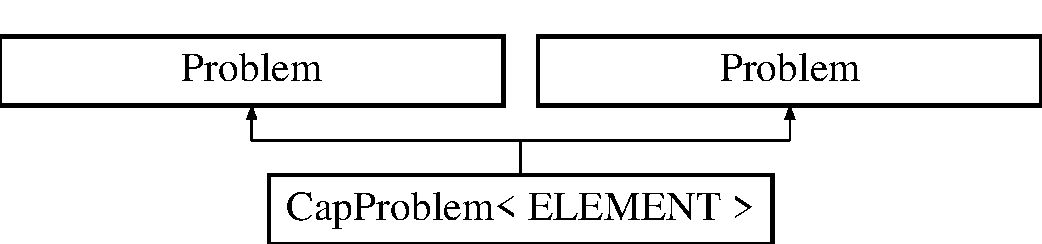
\includegraphics[height=2.000000cm]{classCapProblem}
\end{center}
\end{figure}
\subsection*{Public Member Functions}
\begin{DoxyCompactItemize}
\item 
\hyperlink{classCapProblem_ab03ed8e2c1b44911d11209e00cb28a42}{Cap\+Problem} (const bool \&hijack\+\_\+internal)
\item 
\hyperlink{classCapProblem_ad2b434212ecb33467359aef1071bc964}{$\sim$\+Cap\+Problem} ()
\item 
void \hyperlink{classCapProblem_af54251f12b42b85c6caf88e5214f45da}{parameter\+\_\+study} (const string \&dir\+\_\+name)
\item 
void \hyperlink{classCapProblem_ac852570b51489f4bf744b6063fbfa01a}{actions\+\_\+before\+\_\+newton\+\_\+convergence\+\_\+check} ()
\begin{DoxyCompactList}\small\item\em Update the spine mesh after every Newton step. \end{DoxyCompactList}\item 
void \hyperlink{classCapProblem_aa3a891fe6f5fc5fb5829e3bf636eda2c}{create\+\_\+volume\+\_\+constraint\+\_\+elements} ()
\begin{DoxyCompactList}\small\item\em Create the volume constraint elements. \end{DoxyCompactList}\item 
void \hyperlink{classCapProblem_a8549ca722d2d151ebf3ef7b35b925fbb}{doc\+\_\+solution} (Doc\+Info \&doc\+\_\+info)
\begin{DoxyCompactList}\small\item\em Doc the solution. \end{DoxyCompactList}\end{DoxyCompactItemize}
\subsection*{Private Attributes}
\begin{DoxyCompactItemize}
\item 
double \hyperlink{classCapProblem_ad856df0aa70d881a2b2bc81ad4e2e251}{Ca}
\begin{DoxyCompactList}\small\item\em The Capillary number. \end{DoxyCompactList}\item 
double \hyperlink{classCapProblem_ab1f403fd3be7648c3a52a66684a78f7e}{Volume}
\begin{DoxyCompactList}\small\item\em The volume of the fluid. \end{DoxyCompactList}\item 
double \hyperlink{classCapProblem_a6fcc40a7331c00739923b49c167b396f}{Pext}
\begin{DoxyCompactList}\small\item\em The external pressure. \end{DoxyCompactList}\item 
double \hyperlink{classCapProblem_a7a57e45e3f1b7d30ae9d99bff56e8f5d}{Angle}
\begin{DoxyCompactList}\small\item\em The contact angle. \end{DoxyCompactList}\item 
Single\+Layer\+Spine\+Mesh$<$ Spine\+Element$<$ E\+L\+E\+M\+E\+NT $>$ $>$ $\ast$ \hyperlink{classCapProblem_a6d74594a707d89fc3fd5b87bf1c26a5b}{Bulk\+\_\+mesh\+\_\+pt}
\begin{DoxyCompactList}\small\item\em The bulk mesh of fluid elements. \end{DoxyCompactList}\item 
Mesh $\ast$ \hyperlink{classCapProblem_a557ef36f2db33b81fb3e1828365e66a0}{Surface\+\_\+mesh\+\_\+pt}
\begin{DoxyCompactList}\small\item\em The mesh for the interface elements. \end{DoxyCompactList}\item 
Mesh $\ast$ \hyperlink{classCapProblem_ad1ee833de811bacb3ba3bd9630fe4154}{Point\+\_\+mesh\+\_\+pt}
\begin{DoxyCompactList}\small\item\em The mesh for the element at the contact point. \end{DoxyCompactList}\item 
Mesh $\ast$ \hyperlink{classCapProblem_a4c6655c91412cb031cc2d06ab3ad40f9}{Volume\+\_\+constraint\+\_\+mesh\+\_\+pt}
\begin{DoxyCompactList}\small\item\em The volume constraint mesh. \end{DoxyCompactList}\item 
ofstream \hyperlink{classCapProblem_a46ba6cbe3e82a36db8831fdd53d9f3a9}{Trace\+\_\+file}
\begin{DoxyCompactList}\small\item\em Trace file. \end{DoxyCompactList}\item 
Data $\ast$ \hyperlink{classCapProblem_a3990e9e6a2e4545a470e84ff1fead5eb}{External\+\_\+pressure\+\_\+data\+\_\+pt}
\begin{DoxyCompactList}\small\item\em Data object whose single value stores the external pressure. \end{DoxyCompactList}\item 
Data $\ast$ \hyperlink{classCapProblem_a1ef465adfeb4804ba6e1cd3881c8277b}{Traded\+\_\+pressure\+\_\+data\+\_\+pt}
\begin{DoxyCompactList}\small\item\em Data that is traded for the volume constraint. \end{DoxyCompactList}\end{DoxyCompactItemize}


\subsection{Detailed Description}
\subsubsection*{template$<$class E\+L\+E\+M\+E\+NT$>$\newline
class Cap\+Problem$<$ E\+L\+E\+M\+E\+N\+T $>$}

A Problem class that solves the Navier--Stokes equations + free surface in an axisymmetric geometry using a spine-\/based node update 

Definition at line 81 of file axi\+\_\+static\+\_\+cap.\+cc.



\subsection{Constructor \& Destructor Documentation}
\mbox{\Hypertarget{classCapProblem_ab03ed8e2c1b44911d11209e00cb28a42}\label{classCapProblem_ab03ed8e2c1b44911d11209e00cb28a42}} 
\index{Cap\+Problem@{Cap\+Problem}!Cap\+Problem@{Cap\+Problem}}
\index{Cap\+Problem@{Cap\+Problem}!Cap\+Problem@{Cap\+Problem}}
\subsubsection{\texorpdfstring{Cap\+Problem()}{CapProblem()}}
{\footnotesize\ttfamily template$<$class E\+L\+E\+M\+E\+NT $>$ \\
\hyperlink{classCapProblem}{Cap\+Problem}$<$ E\+L\+E\+M\+E\+NT $>$\+::\hyperlink{classCapProblem}{Cap\+Problem} (\begin{DoxyParamCaption}\item[{const bool \&}]{hijack\+\_\+internal }\end{DoxyParamCaption})}

Constructor\+: Pass boolean flag to indicate if the volume constraint is applied by hijacking an internal pressure or the external pressure 

Definition at line 151 of file axi\+\_\+static\+\_\+cap.\+cc.



References Cap\+Problem$<$ E\+L\+E\+M\+E\+N\+T $>$\+::\+Angle, Cap\+Problem$<$ E\+L\+E\+M\+E\+N\+T $>$\+::\+Bulk\+\_\+mesh\+\_\+pt, Cap\+Problem$<$ E\+L\+E\+M\+E\+N\+T $>$\+::\+Ca, Cap\+Problem$<$ E\+L\+E\+M\+E\+N\+T $>$\+::create\+\_\+volume\+\_\+constraint\+\_\+elements(), Cap\+Problem$<$ E\+L\+E\+M\+E\+N\+T $>$\+::\+External\+\_\+pressure\+\_\+data\+\_\+pt, Cap\+Problem$<$ E\+L\+E\+M\+E\+N\+T $>$\+::\+Pext, Cap\+Problem$<$ E\+L\+E\+M\+E\+N\+T $>$\+::\+Point\+\_\+mesh\+\_\+pt, Cap\+Problem$<$ E\+L\+E\+M\+E\+N\+T $>$\+::\+Surface\+\_\+mesh\+\_\+pt, Cap\+Problem$<$ E\+L\+E\+M\+E\+N\+T $>$\+::\+Traded\+\_\+pressure\+\_\+data\+\_\+pt, Cap\+Problem$<$ E\+L\+E\+M\+E\+N\+T $>$\+::\+Volume\+\_\+constraint\+\_\+mesh\+\_\+pt, Global\+\_\+\+Physical\+\_\+\+Variables\+::\+Wall\+\_\+normal, and Global\+\_\+\+Physical\+\_\+\+Variables\+::wall\+\_\+unit\+\_\+normal\+\_\+fct().

\mbox{\Hypertarget{classCapProblem_ad2b434212ecb33467359aef1071bc964}\label{classCapProblem_ad2b434212ecb33467359aef1071bc964}} 
\index{Cap\+Problem@{Cap\+Problem}!````~Cap\+Problem@{$\sim$\+Cap\+Problem}}
\index{````~Cap\+Problem@{$\sim$\+Cap\+Problem}!Cap\+Problem@{Cap\+Problem}}
\subsubsection{\texorpdfstring{$\sim$\+Cap\+Problem()}{~CapProblem()}}
{\footnotesize\ttfamily template$<$class E\+L\+E\+M\+E\+NT $>$ \\
\hyperlink{classCapProblem}{Cap\+Problem}$<$ E\+L\+E\+M\+E\+NT $>$\+::$\sim$\hyperlink{classCapProblem}{Cap\+Problem} (\begin{DoxyParamCaption}{ }\end{DoxyParamCaption})}

Destructor. Make sure to clean up all allocated memory, so that multiple instances of the problem don\textquotesingle{}t lead to excessive memory usage. 

Definition at line 336 of file axi\+\_\+static\+\_\+cap.\+cc.



References Cap\+Problem$<$ E\+L\+E\+M\+E\+N\+T $>$\+::\+Bulk\+\_\+mesh\+\_\+pt, Cap\+Problem$<$ E\+L\+E\+M\+E\+N\+T $>$\+::\+External\+\_\+pressure\+\_\+data\+\_\+pt, Cap\+Problem$<$ E\+L\+E\+M\+E\+N\+T $>$\+::\+Point\+\_\+mesh\+\_\+pt, Cap\+Problem$<$ E\+L\+E\+M\+E\+N\+T $>$\+::\+Surface\+\_\+mesh\+\_\+pt, Cap\+Problem$<$ E\+L\+E\+M\+E\+N\+T $>$\+::\+Traded\+\_\+pressure\+\_\+data\+\_\+pt, and Cap\+Problem$<$ E\+L\+E\+M\+E\+N\+T $>$\+::\+Volume\+\_\+constraint\+\_\+mesh\+\_\+pt.



\subsection{Member Function Documentation}
\mbox{\Hypertarget{classCapProblem_ac852570b51489f4bf744b6063fbfa01a}\label{classCapProblem_ac852570b51489f4bf744b6063fbfa01a}} 
\index{Cap\+Problem@{Cap\+Problem}!actions\+\_\+before\+\_\+newton\+\_\+convergence\+\_\+check@{actions\+\_\+before\+\_\+newton\+\_\+convergence\+\_\+check}}
\index{actions\+\_\+before\+\_\+newton\+\_\+convergence\+\_\+check@{actions\+\_\+before\+\_\+newton\+\_\+convergence\+\_\+check}!Cap\+Problem@{Cap\+Problem}}
\subsubsection{\texorpdfstring{actions\+\_\+before\+\_\+newton\+\_\+convergence\+\_\+check()}{actions\_before\_newton\_convergence\_check()}}
{\footnotesize\ttfamily template$<$class E\+L\+E\+M\+E\+NT$>$ \\
void \hyperlink{classCapProblem}{Cap\+Problem}$<$ E\+L\+E\+M\+E\+NT $>$\+::actions\+\_\+before\+\_\+newton\+\_\+convergence\+\_\+check (\begin{DoxyParamCaption}{ }\end{DoxyParamCaption})\hspace{0.3cm}{\ttfamily [inline]}}



Update the spine mesh after every Newton step. 



Definition at line 98 of file axi\+\_\+static\+\_\+cap.\+cc.

\mbox{\Hypertarget{classCapProblem_aa3a891fe6f5fc5fb5829e3bf636eda2c}\label{classCapProblem_aa3a891fe6f5fc5fb5829e3bf636eda2c}} 
\index{Cap\+Problem@{Cap\+Problem}!create\+\_\+volume\+\_\+constraint\+\_\+elements@{create\+\_\+volume\+\_\+constraint\+\_\+elements}}
\index{create\+\_\+volume\+\_\+constraint\+\_\+elements@{create\+\_\+volume\+\_\+constraint\+\_\+elements}!Cap\+Problem@{Cap\+Problem}}
\subsubsection{\texorpdfstring{create\+\_\+volume\+\_\+constraint\+\_\+elements()}{create\_volume\_constraint\_elements()}}
{\footnotesize\ttfamily template$<$class E\+L\+E\+M\+E\+NT $>$ \\
void \hyperlink{classCapProblem}{Cap\+Problem}$<$ E\+L\+E\+M\+E\+NT $>$\+::create\+\_\+volume\+\_\+constraint\+\_\+elements (\begin{DoxyParamCaption}{ }\end{DoxyParamCaption})}



Create the volume constraint elements. 



Definition at line 380 of file axi\+\_\+static\+\_\+cap.\+cc.



References Cap\+Problem$<$ E\+L\+E\+M\+E\+N\+T $>$\+::\+Bulk\+\_\+mesh\+\_\+pt, Cap\+Problem$<$ E\+L\+E\+M\+E\+N\+T $>$\+::\+Traded\+\_\+pressure\+\_\+data\+\_\+pt, Cap\+Problem$<$ E\+L\+E\+M\+E\+N\+T $>$\+::\+Volume, and Cap\+Problem$<$ E\+L\+E\+M\+E\+N\+T $>$\+::\+Volume\+\_\+constraint\+\_\+mesh\+\_\+pt.



Referenced by Cap\+Problem$<$ E\+L\+E\+M\+E\+N\+T $>$\+::\+Cap\+Problem().

\mbox{\Hypertarget{classCapProblem_a8549ca722d2d151ebf3ef7b35b925fbb}\label{classCapProblem_a8549ca722d2d151ebf3ef7b35b925fbb}} 
\index{Cap\+Problem@{Cap\+Problem}!doc\+\_\+solution@{doc\+\_\+solution}}
\index{doc\+\_\+solution@{doc\+\_\+solution}!Cap\+Problem@{Cap\+Problem}}
\subsubsection{\texorpdfstring{doc\+\_\+solution()}{doc\_solution()}}
{\footnotesize\ttfamily template$<$class E\+L\+E\+M\+E\+NT $>$ \\
void \hyperlink{classCapProblem}{Cap\+Problem}$<$ E\+L\+E\+M\+E\+NT $>$\+::doc\+\_\+solution (\begin{DoxyParamCaption}\item[{Doc\+Info \&}]{doc\+\_\+info }\end{DoxyParamCaption})}



Doc the solution. 



Definition at line 469 of file axi\+\_\+static\+\_\+cap.\+cc.



References Cap\+Problem$<$ E\+L\+E\+M\+E\+N\+T $>$\+::\+Angle, Cap\+Problem$<$ E\+L\+E\+M\+E\+N\+T $>$\+::\+Bulk\+\_\+mesh\+\_\+pt, Cap\+Problem$<$ E\+L\+E\+M\+E\+N\+T $>$\+::\+Ca, Cap\+Problem$<$ E\+L\+E\+M\+E\+N\+T $>$\+::\+External\+\_\+pressure\+\_\+data\+\_\+pt, Cap\+Problem$<$ E\+L\+E\+M\+E\+N\+T $>$\+::\+Surface\+\_\+mesh\+\_\+pt, and Cap\+Problem$<$ E\+L\+E\+M\+E\+N\+T $>$\+::\+Trace\+\_\+file.



Referenced by Cap\+Problem$<$ E\+L\+E\+M\+E\+N\+T $>$\+::parameter\+\_\+study().

\mbox{\Hypertarget{classCapProblem_af54251f12b42b85c6caf88e5214f45da}\label{classCapProblem_af54251f12b42b85c6caf88e5214f45da}} 
\index{Cap\+Problem@{Cap\+Problem}!parameter\+\_\+study@{parameter\+\_\+study}}
\index{parameter\+\_\+study@{parameter\+\_\+study}!Cap\+Problem@{Cap\+Problem}}
\subsubsection{\texorpdfstring{parameter\+\_\+study()}{parameter\_study()}}
{\footnotesize\ttfamily template$<$class E\+L\+E\+M\+E\+NT $>$ \\
void \hyperlink{classCapProblem}{Cap\+Problem}$<$ E\+L\+E\+M\+E\+NT $>$\+::parameter\+\_\+study (\begin{DoxyParamCaption}\item[{const string \&}]{dir\+\_\+name }\end{DoxyParamCaption})}

Perform a parameter study\+: Solve problem for a range of contact angles Pass name of output directory as a string

Perform a parameter study. Pass name of output directory as a string 

Definition at line 425 of file axi\+\_\+static\+\_\+cap.\+cc.



References Cap\+Problem$<$ E\+L\+E\+M\+E\+N\+T $>$\+::\+Angle, Cap\+Problem$<$ E\+L\+E\+M\+E\+N\+T $>$\+::doc\+\_\+solution(), and Cap\+Problem$<$ E\+L\+E\+M\+E\+N\+T $>$\+::\+Trace\+\_\+file.



Referenced by main().



\subsection{Member Data Documentation}
\mbox{\Hypertarget{classCapProblem_a7a57e45e3f1b7d30ae9d99bff56e8f5d}\label{classCapProblem_a7a57e45e3f1b7d30ae9d99bff56e8f5d}} 
\index{Cap\+Problem@{Cap\+Problem}!Angle@{Angle}}
\index{Angle@{Angle}!Cap\+Problem@{Cap\+Problem}}
\subsubsection{\texorpdfstring{Angle}{Angle}}
{\footnotesize\ttfamily template$<$class E\+L\+E\+M\+E\+NT$>$ \\
double \hyperlink{classCapProblem}{Cap\+Problem}$<$ E\+L\+E\+M\+E\+NT $>$\+::Angle\hspace{0.3cm}{\ttfamily [private]}}



The contact angle. 



Definition at line 118 of file axi\+\_\+static\+\_\+cap.\+cc.



Referenced by Cap\+Problem$<$ E\+L\+E\+M\+E\+N\+T $>$\+::\+Cap\+Problem(), Cap\+Problem$<$ E\+L\+E\+M\+E\+N\+T $>$\+::doc\+\_\+solution(), and Cap\+Problem$<$ E\+L\+E\+M\+E\+N\+T $>$\+::parameter\+\_\+study().

\mbox{\Hypertarget{classCapProblem_a6d74594a707d89fc3fd5b87bf1c26a5b}\label{classCapProblem_a6d74594a707d89fc3fd5b87bf1c26a5b}} 
\index{Cap\+Problem@{Cap\+Problem}!Bulk\+\_\+mesh\+\_\+pt@{Bulk\+\_\+mesh\+\_\+pt}}
\index{Bulk\+\_\+mesh\+\_\+pt@{Bulk\+\_\+mesh\+\_\+pt}!Cap\+Problem@{Cap\+Problem}}
\subsubsection{\texorpdfstring{Bulk\+\_\+mesh\+\_\+pt}{Bulk\_mesh\_pt}}
{\footnotesize\ttfamily template$<$class E\+L\+E\+M\+E\+NT$>$ \\
Single\+Layer\+Spine\+Mesh$<$Spine\+Element$<$E\+L\+E\+M\+E\+NT$>$ $>$$\ast$ \hyperlink{classCapProblem}{Cap\+Problem}$<$ E\+L\+E\+M\+E\+NT $>$\+::Bulk\+\_\+mesh\+\_\+pt\hspace{0.3cm}{\ttfamily [private]}}



The bulk mesh of fluid elements. 



Definition at line 121 of file axi\+\_\+static\+\_\+cap.\+cc.



Referenced by Cap\+Problem$<$ E\+L\+E\+M\+E\+N\+T $>$\+::\+Cap\+Problem(), Cap\+Problem$<$ E\+L\+E\+M\+E\+N\+T $>$\+::create\+\_\+volume\+\_\+constraint\+\_\+elements(), Cap\+Problem$<$ E\+L\+E\+M\+E\+N\+T $>$\+::doc\+\_\+solution(), and Cap\+Problem$<$ E\+L\+E\+M\+E\+N\+T $>$\+::$\sim$\+Cap\+Problem().

\mbox{\Hypertarget{classCapProblem_ad856df0aa70d881a2b2bc81ad4e2e251}\label{classCapProblem_ad856df0aa70d881a2b2bc81ad4e2e251}} 
\index{Cap\+Problem@{Cap\+Problem}!Ca@{Ca}}
\index{Ca@{Ca}!Cap\+Problem@{Cap\+Problem}}
\subsubsection{\texorpdfstring{Ca}{Ca}}
{\footnotesize\ttfamily template$<$class E\+L\+E\+M\+E\+NT$>$ \\
double \hyperlink{classCapProblem}{Cap\+Problem}$<$ E\+L\+E\+M\+E\+NT $>$\+::Ca\hspace{0.3cm}{\ttfamily [private]}}



The Capillary number. 



Definition at line 109 of file axi\+\_\+static\+\_\+cap.\+cc.



Referenced by Cap\+Problem$<$ E\+L\+E\+M\+E\+N\+T $>$\+::\+Cap\+Problem(), and Cap\+Problem$<$ E\+L\+E\+M\+E\+N\+T $>$\+::doc\+\_\+solution().

\mbox{\Hypertarget{classCapProblem_a3990e9e6a2e4545a470e84ff1fead5eb}\label{classCapProblem_a3990e9e6a2e4545a470e84ff1fead5eb}} 
\index{Cap\+Problem@{Cap\+Problem}!External\+\_\+pressure\+\_\+data\+\_\+pt@{External\+\_\+pressure\+\_\+data\+\_\+pt}}
\index{External\+\_\+pressure\+\_\+data\+\_\+pt@{External\+\_\+pressure\+\_\+data\+\_\+pt}!Cap\+Problem@{Cap\+Problem}}
\subsubsection{\texorpdfstring{External\+\_\+pressure\+\_\+data\+\_\+pt}{External\_pressure\_data\_pt}}
{\footnotesize\ttfamily template$<$class E\+L\+E\+M\+E\+NT$>$ \\
Data$\ast$ \hyperlink{classCapProblem}{Cap\+Problem}$<$ E\+L\+E\+M\+E\+NT $>$\+::External\+\_\+pressure\+\_\+data\+\_\+pt\hspace{0.3cm}{\ttfamily [private]}}



Data object whose single value stores the external pressure. 



Definition at line 136 of file axi\+\_\+static\+\_\+cap.\+cc.



Referenced by Cap\+Problem$<$ E\+L\+E\+M\+E\+N\+T $>$\+::\+Cap\+Problem(), Cap\+Problem$<$ E\+L\+E\+M\+E\+N\+T $>$\+::doc\+\_\+solution(), and Cap\+Problem$<$ E\+L\+E\+M\+E\+N\+T $>$\+::$\sim$\+Cap\+Problem().

\mbox{\Hypertarget{classCapProblem_a6fcc40a7331c00739923b49c167b396f}\label{classCapProblem_a6fcc40a7331c00739923b49c167b396f}} 
\index{Cap\+Problem@{Cap\+Problem}!Pext@{Pext}}
\index{Pext@{Pext}!Cap\+Problem@{Cap\+Problem}}
\subsubsection{\texorpdfstring{Pext}{Pext}}
{\footnotesize\ttfamily template$<$class E\+L\+E\+M\+E\+NT$>$ \\
double \hyperlink{classCapProblem}{Cap\+Problem}$<$ E\+L\+E\+M\+E\+NT $>$\+::Pext\hspace{0.3cm}{\ttfamily [private]}}



The external pressure. 



Definition at line 115 of file axi\+\_\+static\+\_\+cap.\+cc.



Referenced by Cap\+Problem$<$ E\+L\+E\+M\+E\+N\+T $>$\+::\+Cap\+Problem().

\mbox{\Hypertarget{classCapProblem_ad1ee833de811bacb3ba3bd9630fe4154}\label{classCapProblem_ad1ee833de811bacb3ba3bd9630fe4154}} 
\index{Cap\+Problem@{Cap\+Problem}!Point\+\_\+mesh\+\_\+pt@{Point\+\_\+mesh\+\_\+pt}}
\index{Point\+\_\+mesh\+\_\+pt@{Point\+\_\+mesh\+\_\+pt}!Cap\+Problem@{Cap\+Problem}}
\subsubsection{\texorpdfstring{Point\+\_\+mesh\+\_\+pt}{Point\_mesh\_pt}}
{\footnotesize\ttfamily template$<$class E\+L\+E\+M\+E\+NT$>$ \\
Mesh$\ast$ \hyperlink{classCapProblem}{Cap\+Problem}$<$ E\+L\+E\+M\+E\+NT $>$\+::Point\+\_\+mesh\+\_\+pt\hspace{0.3cm}{\ttfamily [private]}}



The mesh for the element at the contact point. 



Definition at line 127 of file axi\+\_\+static\+\_\+cap.\+cc.



Referenced by Cap\+Problem$<$ E\+L\+E\+M\+E\+N\+T $>$\+::\+Cap\+Problem(), and Cap\+Problem$<$ E\+L\+E\+M\+E\+N\+T $>$\+::$\sim$\+Cap\+Problem().

\mbox{\Hypertarget{classCapProblem_a557ef36f2db33b81fb3e1828365e66a0}\label{classCapProblem_a557ef36f2db33b81fb3e1828365e66a0}} 
\index{Cap\+Problem@{Cap\+Problem}!Surface\+\_\+mesh\+\_\+pt@{Surface\+\_\+mesh\+\_\+pt}}
\index{Surface\+\_\+mesh\+\_\+pt@{Surface\+\_\+mesh\+\_\+pt}!Cap\+Problem@{Cap\+Problem}}
\subsubsection{\texorpdfstring{Surface\+\_\+mesh\+\_\+pt}{Surface\_mesh\_pt}}
{\footnotesize\ttfamily template$<$class E\+L\+E\+M\+E\+NT$>$ \\
Mesh$\ast$ \hyperlink{classCapProblem}{Cap\+Problem}$<$ E\+L\+E\+M\+E\+NT $>$\+::Surface\+\_\+mesh\+\_\+pt\hspace{0.3cm}{\ttfamily [private]}}



The mesh for the interface elements. 



Definition at line 124 of file axi\+\_\+static\+\_\+cap.\+cc.



Referenced by Cap\+Problem$<$ E\+L\+E\+M\+E\+N\+T $>$\+::\+Cap\+Problem(), Cap\+Problem$<$ E\+L\+E\+M\+E\+N\+T $>$\+::doc\+\_\+solution(), and Cap\+Problem$<$ E\+L\+E\+M\+E\+N\+T $>$\+::$\sim$\+Cap\+Problem().

\mbox{\Hypertarget{classCapProblem_a46ba6cbe3e82a36db8831fdd53d9f3a9}\label{classCapProblem_a46ba6cbe3e82a36db8831fdd53d9f3a9}} 
\index{Cap\+Problem@{Cap\+Problem}!Trace\+\_\+file@{Trace\+\_\+file}}
\index{Trace\+\_\+file@{Trace\+\_\+file}!Cap\+Problem@{Cap\+Problem}}
\subsubsection{\texorpdfstring{Trace\+\_\+file}{Trace\_file}}
{\footnotesize\ttfamily template$<$class E\+L\+E\+M\+E\+NT$>$ \\
ofstream \hyperlink{classCapProblem}{Cap\+Problem}$<$ E\+L\+E\+M\+E\+NT $>$\+::Trace\+\_\+file\hspace{0.3cm}{\ttfamily [private]}}



Trace file. 



Definition at line 133 of file axi\+\_\+static\+\_\+cap.\+cc.



Referenced by Cap\+Problem$<$ E\+L\+E\+M\+E\+N\+T $>$\+::doc\+\_\+solution(), and Cap\+Problem$<$ E\+L\+E\+M\+E\+N\+T $>$\+::parameter\+\_\+study().

\mbox{\Hypertarget{classCapProblem_a1ef465adfeb4804ba6e1cd3881c8277b}\label{classCapProblem_a1ef465adfeb4804ba6e1cd3881c8277b}} 
\index{Cap\+Problem@{Cap\+Problem}!Traded\+\_\+pressure\+\_\+data\+\_\+pt@{Traded\+\_\+pressure\+\_\+data\+\_\+pt}}
\index{Traded\+\_\+pressure\+\_\+data\+\_\+pt@{Traded\+\_\+pressure\+\_\+data\+\_\+pt}!Cap\+Problem@{Cap\+Problem}}
\subsubsection{\texorpdfstring{Traded\+\_\+pressure\+\_\+data\+\_\+pt}{Traded\_pressure\_data\_pt}}
{\footnotesize\ttfamily template$<$class E\+L\+E\+M\+E\+NT$>$ \\
Data$\ast$ \hyperlink{classCapProblem}{Cap\+Problem}$<$ E\+L\+E\+M\+E\+NT $>$\+::Traded\+\_\+pressure\+\_\+data\+\_\+pt\hspace{0.3cm}{\ttfamily [private]}}



Data that is traded for the volume constraint. 



Definition at line 139 of file axi\+\_\+static\+\_\+cap.\+cc.



Referenced by Cap\+Problem$<$ E\+L\+E\+M\+E\+N\+T $>$\+::\+Cap\+Problem(), Cap\+Problem$<$ E\+L\+E\+M\+E\+N\+T $>$\+::create\+\_\+volume\+\_\+constraint\+\_\+elements(), and Cap\+Problem$<$ E\+L\+E\+M\+E\+N\+T $>$\+::$\sim$\+Cap\+Problem().

\mbox{\Hypertarget{classCapProblem_ab1f403fd3be7648c3a52a66684a78f7e}\label{classCapProblem_ab1f403fd3be7648c3a52a66684a78f7e}} 
\index{Cap\+Problem@{Cap\+Problem}!Volume@{Volume}}
\index{Volume@{Volume}!Cap\+Problem@{Cap\+Problem}}
\subsubsection{\texorpdfstring{Volume}{Volume}}
{\footnotesize\ttfamily template$<$class E\+L\+E\+M\+E\+NT$>$ \\
double \hyperlink{classCapProblem}{Cap\+Problem}$<$ E\+L\+E\+M\+E\+NT $>$\+::Volume\hspace{0.3cm}{\ttfamily [private]}}



The volume of the fluid. 



Definition at line 112 of file axi\+\_\+static\+\_\+cap.\+cc.



Referenced by Cap\+Problem$<$ E\+L\+E\+M\+E\+N\+T $>$\+::create\+\_\+volume\+\_\+constraint\+\_\+elements().

\mbox{\Hypertarget{classCapProblem_a4c6655c91412cb031cc2d06ab3ad40f9}\label{classCapProblem_a4c6655c91412cb031cc2d06ab3ad40f9}} 
\index{Cap\+Problem@{Cap\+Problem}!Volume\+\_\+constraint\+\_\+mesh\+\_\+pt@{Volume\+\_\+constraint\+\_\+mesh\+\_\+pt}}
\index{Volume\+\_\+constraint\+\_\+mesh\+\_\+pt@{Volume\+\_\+constraint\+\_\+mesh\+\_\+pt}!Cap\+Problem@{Cap\+Problem}}
\subsubsection{\texorpdfstring{Volume\+\_\+constraint\+\_\+mesh\+\_\+pt}{Volume\_constraint\_mesh\_pt}}
{\footnotesize\ttfamily template$<$class E\+L\+E\+M\+E\+NT$>$ \\
Mesh$\ast$ \hyperlink{classCapProblem}{Cap\+Problem}$<$ E\+L\+E\+M\+E\+NT $>$\+::Volume\+\_\+constraint\+\_\+mesh\+\_\+pt\hspace{0.3cm}{\ttfamily [private]}}



The volume constraint mesh. 



Definition at line 130 of file axi\+\_\+static\+\_\+cap.\+cc.



Referenced by Cap\+Problem$<$ E\+L\+E\+M\+E\+N\+T $>$\+::\+Cap\+Problem(), Cap\+Problem$<$ E\+L\+E\+M\+E\+N\+T $>$\+::create\+\_\+volume\+\_\+constraint\+\_\+elements(), and Cap\+Problem$<$ E\+L\+E\+M\+E\+N\+T $>$\+::$\sim$\+Cap\+Problem().



The documentation for this class was generated from the following file\+:\begin{DoxyCompactItemize}
\item 
\hyperlink{axi__static__cap_8cc}{axi\+\_\+static\+\_\+cap.\+cc}\end{DoxyCompactItemize}

\hypertarget{classElasticTwoLayerMesh}{}\section{Elastic\+Two\+Layer\+Mesh$<$ E\+L\+E\+M\+E\+NT $>$ Class Template Reference}
\label{classElasticTwoLayerMesh}\index{Elastic\+Two\+Layer\+Mesh$<$ E\+L\+E\+M\+E\+N\+T $>$@{Elastic\+Two\+Layer\+Mesh$<$ E\+L\+E\+M\+E\+N\+T $>$}}
Inheritance diagram for Elastic\+Two\+Layer\+Mesh$<$ E\+L\+E\+M\+E\+NT $>$\+:\begin{figure}[H]
\begin{center}
\leavevmode
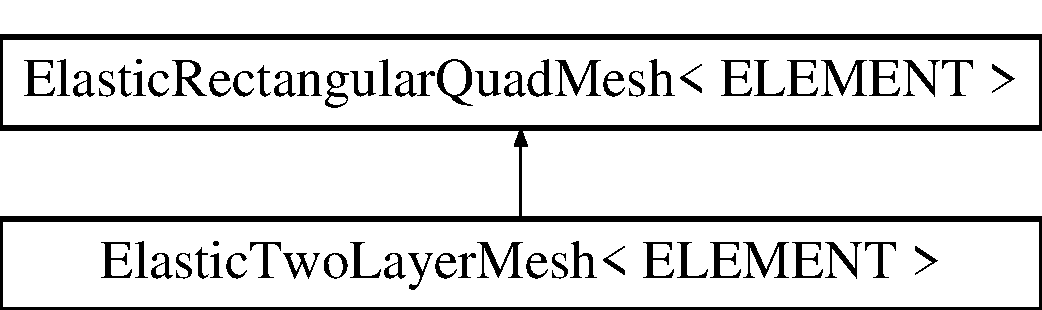
\includegraphics[height=2.000000cm]{classElasticTwoLayerMesh}
\end{center}
\end{figure}
\subsection*{Public Member Functions}
\begin{DoxyCompactItemize}
\item 
\hyperlink{classElasticTwoLayerMesh_a720be7cd7b0f44df04dcb0d09a2795a7}{Elastic\+Two\+Layer\+Mesh} (const unsigned \&nx, const unsigned \&ny1, const unsigned \&ny2, const double \&lx, const double \&h1, const double \&h2, const bool \&periodic\+\_\+in\+\_\+x=false, Time\+Stepper $\ast$time\+\_\+stepper\+\_\+pt=\&Mesh\+::\+Default\+\_\+\+Time\+Stepper)
\begin{DoxyCompactList}\small\item\em Constructor\+: Pass number of elements in x-\/direction, number of elements in y-\/direction in bottom and top layer, respectively, axial length and height of top and bottom layers, a boolean flag to make the mesh periodic in the x-\/direction, and pointer to timestepper (defaults to Steady timestepper) \end{DoxyCompactList}\item 
Finite\+Element $\ast$\& \hyperlink{classElasticTwoLayerMesh_ab5b2682b701b796c14431f8e126457fd}{upper\+\_\+layer\+\_\+element\+\_\+pt} (const unsigned long \&i)
\begin{DoxyCompactList}\small\item\em Access functions for pointers to elements in upper layer. \end{DoxyCompactList}\item 
Finite\+Element $\ast$\& \hyperlink{classElasticTwoLayerMesh_a4e6d9b26eecc0487d7b2684ad27b7669}{lower\+\_\+layer\+\_\+element\+\_\+pt} (const unsigned long \&i)
\begin{DoxyCompactList}\small\item\em Access functions for pointers to elements in bottom layer. \end{DoxyCompactList}\item 
unsigned long \hyperlink{classElasticTwoLayerMesh_ae5c586ecab2ac275174427a94ccfc0c7}{nupper} () const
\begin{DoxyCompactList}\small\item\em Number of elements in upper layer. \end{DoxyCompactList}\item 
unsigned long \hyperlink{classElasticTwoLayerMesh_a144f4d44005a25bb301955625a79c9ef}{nlower} () const
\begin{DoxyCompactList}\small\item\em Number of elements in top layer. \end{DoxyCompactList}\item 
Finite\+Element $\ast$\& \hyperlink{classElasticTwoLayerMesh_a5170e0a70ad0d4eb3ec01c32d3db2c72}{interface\+\_\+upper\+\_\+boundary\+\_\+element\+\_\+pt} (const unsigned long \&i)
\begin{DoxyCompactList}\small\item\em Access functions for pointers to elements in upper layer. \end{DoxyCompactList}\item 
Finite\+Element $\ast$\& \hyperlink{classElasticTwoLayerMesh_a748ff5229092301a18a193a846d2ebdd}{interface\+\_\+lower\+\_\+boundary\+\_\+element\+\_\+pt} (const unsigned long \&i)
\begin{DoxyCompactList}\small\item\em Access functions for pointers to elements in bottom layer. \end{DoxyCompactList}\item 
unsigned long \hyperlink{classElasticTwoLayerMesh_a6e813329601844d3d900d78a60892134}{ninterface\+\_\+upper} () const
\begin{DoxyCompactList}\small\item\em Number of elements in upper layer. \end{DoxyCompactList}\item 
unsigned long \hyperlink{classElasticTwoLayerMesh_ae5db5553497593905fd227bfc5b34b50}{ninterface\+\_\+lower} () const
\begin{DoxyCompactList}\small\item\em Number of elements in top layer. \end{DoxyCompactList}\item 
int \hyperlink{classElasticTwoLayerMesh_a074aafe34f7dd56566c1a9ff934505d5}{interface\+\_\+upper\+\_\+face\+\_\+index\+\_\+at\+\_\+boundary} (const unsigned \&e)
\begin{DoxyCompactList}\small\item\em Index of the face of the elements next to the interface in the upper region (always -\/2) \end{DoxyCompactList}\item 
int \hyperlink{classElasticTwoLayerMesh_a100b3b26d4a2b97f67b0bef4e4b42e64}{interface\+\_\+lower\+\_\+face\+\_\+index\+\_\+at\+\_\+boundary} (const unsigned \&e)
\begin{DoxyCompactList}\small\item\em Index of the face of the elements next to the interface in the lower region (always 2) \end{DoxyCompactList}\end{DoxyCompactItemize}
\subsection*{Private Attributes}
\begin{DoxyCompactItemize}
\item 
Vector$<$ Finite\+Element $\ast$ $>$ \hyperlink{classElasticTwoLayerMesh_a4f8c33eaaa185e8c8710883ee9b5811f}{Lower\+\_\+layer\+\_\+element\+\_\+pt}
\begin{DoxyCompactList}\small\item\em Vector of pointers to element in the upper layer. \end{DoxyCompactList}\item 
Vector$<$ Finite\+Element $\ast$ $>$ \hyperlink{classElasticTwoLayerMesh_ae46d4ef2bb95a6c023bd0dc1e367ccfb}{Upper\+\_\+layer\+\_\+element\+\_\+pt}
\begin{DoxyCompactList}\small\item\em Vector of pointers to element in the lower layer. \end{DoxyCompactList}\item 
Vector$<$ Finite\+Element $\ast$ $>$ \hyperlink{classElasticTwoLayerMesh_abc8751d632399afe56df6c32e1001582}{Interface\+\_\+lower\+\_\+boundary\+\_\+element\+\_\+pt}
\begin{DoxyCompactList}\small\item\em Vector of pointers to the elements adjacent to the interface on the lower layer. \end{DoxyCompactList}\item 
Vector$<$ Finite\+Element $\ast$ $>$ \hyperlink{classElasticTwoLayerMesh_af8218bd023535d3dbf4af3cf7bc1c12d}{Interface\+\_\+upper\+\_\+boundary\+\_\+element\+\_\+pt}
\begin{DoxyCompactList}\small\item\em Vector of pointers to the element adjacent to the interface on the upper layer. \end{DoxyCompactList}\end{DoxyCompactItemize}


\subsection{Detailed Description}
\subsubsection*{template$<$class E\+L\+E\+M\+E\+NT$>$\newline
class Elastic\+Two\+Layer\+Mesh$<$ E\+L\+E\+M\+E\+N\+T $>$}

Two layer mesh which employs a pseudo-\/solid node-\/update strategy. This class is essentially a wrapper to an Elastic\+Rectangular\+Quad\+Mesh, with an additional boundary to represent the interface between the two fluid layers. In addition, the mesh paritions the elements into those above and below the interface and relabels boundaries so that we can impose a volume constraint on the lower or upper fluid. \begin{DoxyVerb}                            3
          ---------------------------------------
          |                                     |
        4 |                                     | 2
          |                 6                   |
          ---------------------------------------
          |                                     |
        5 |                                     | 1
          |                                     |
          ---------------------------------------
                            0  \end{DoxyVerb}
 

Definition at line 456 of file static\+\_\+two\+\_\+layer.\+cc.



\subsection{Constructor \& Destructor Documentation}
\mbox{\Hypertarget{classElasticTwoLayerMesh_a720be7cd7b0f44df04dcb0d09a2795a7}\label{classElasticTwoLayerMesh_a720be7cd7b0f44df04dcb0d09a2795a7}} 
\index{Elastic\+Two\+Layer\+Mesh@{Elastic\+Two\+Layer\+Mesh}!Elastic\+Two\+Layer\+Mesh@{Elastic\+Two\+Layer\+Mesh}}
\index{Elastic\+Two\+Layer\+Mesh@{Elastic\+Two\+Layer\+Mesh}!Elastic\+Two\+Layer\+Mesh@{Elastic\+Two\+Layer\+Mesh}}
\subsubsection{\texorpdfstring{Elastic\+Two\+Layer\+Mesh()}{ElasticTwoLayerMesh()}}
{\footnotesize\ttfamily template$<$class E\+L\+E\+M\+E\+NT$>$ \\
\hyperlink{classElasticTwoLayerMesh}{Elastic\+Two\+Layer\+Mesh}$<$ E\+L\+E\+M\+E\+NT $>$\+::\hyperlink{classElasticTwoLayerMesh}{Elastic\+Two\+Layer\+Mesh} (\begin{DoxyParamCaption}\item[{const unsigned \&}]{nx,  }\item[{const unsigned \&}]{ny1,  }\item[{const unsigned \&}]{ny2,  }\item[{const double \&}]{lx,  }\item[{const double \&}]{h1,  }\item[{const double \&}]{h2,  }\item[{const bool \&}]{periodic\+\_\+in\+\_\+x = {\ttfamily false},  }\item[{Time\+Stepper $\ast$}]{time\+\_\+stepper\+\_\+pt = {\ttfamily \&Mesh\+:\+:Default\+\_\+TimeStepper} }\end{DoxyParamCaption})\hspace{0.3cm}{\ttfamily [inline]}}



Constructor\+: Pass number of elements in x-\/direction, number of elements in y-\/direction in bottom and top layer, respectively, axial length and height of top and bottom layers, a boolean flag to make the mesh periodic in the x-\/direction, and pointer to timestepper (defaults to Steady timestepper) 



Definition at line 467 of file static\+\_\+two\+\_\+layer.\+cc.



\subsection{Member Function Documentation}
\mbox{\Hypertarget{classElasticTwoLayerMesh_a748ff5229092301a18a193a846d2ebdd}\label{classElasticTwoLayerMesh_a748ff5229092301a18a193a846d2ebdd}} 
\index{Elastic\+Two\+Layer\+Mesh@{Elastic\+Two\+Layer\+Mesh}!interface\+\_\+lower\+\_\+boundary\+\_\+element\+\_\+pt@{interface\+\_\+lower\+\_\+boundary\+\_\+element\+\_\+pt}}
\index{interface\+\_\+lower\+\_\+boundary\+\_\+element\+\_\+pt@{interface\+\_\+lower\+\_\+boundary\+\_\+element\+\_\+pt}!Elastic\+Two\+Layer\+Mesh@{Elastic\+Two\+Layer\+Mesh}}
\subsubsection{\texorpdfstring{interface\+\_\+lower\+\_\+boundary\+\_\+element\+\_\+pt()}{interface\_lower\_boundary\_element\_pt()}}
{\footnotesize\ttfamily template$<$class E\+L\+E\+M\+E\+NT$>$ \\
Finite\+Element$\ast$ \& \hyperlink{classElasticTwoLayerMesh}{Elastic\+Two\+Layer\+Mesh}$<$ E\+L\+E\+M\+E\+NT $>$\+::interface\+\_\+lower\+\_\+boundary\+\_\+element\+\_\+pt (\begin{DoxyParamCaption}\item[{const unsigned long \&}]{i }\end{DoxyParamCaption})\hspace{0.3cm}{\ttfamily [inline]}}



Access functions for pointers to elements in bottom layer. 



Definition at line 705 of file static\+\_\+two\+\_\+layer.\+cc.

\mbox{\Hypertarget{classElasticTwoLayerMesh_a100b3b26d4a2b97f67b0bef4e4b42e64}\label{classElasticTwoLayerMesh_a100b3b26d4a2b97f67b0bef4e4b42e64}} 
\index{Elastic\+Two\+Layer\+Mesh@{Elastic\+Two\+Layer\+Mesh}!interface\+\_\+lower\+\_\+face\+\_\+index\+\_\+at\+\_\+boundary@{interface\+\_\+lower\+\_\+face\+\_\+index\+\_\+at\+\_\+boundary}}
\index{interface\+\_\+lower\+\_\+face\+\_\+index\+\_\+at\+\_\+boundary@{interface\+\_\+lower\+\_\+face\+\_\+index\+\_\+at\+\_\+boundary}!Elastic\+Two\+Layer\+Mesh@{Elastic\+Two\+Layer\+Mesh}}
\subsubsection{\texorpdfstring{interface\+\_\+lower\+\_\+face\+\_\+index\+\_\+at\+\_\+boundary()}{interface\_lower\_face\_index\_at\_boundary()}}
{\footnotesize\ttfamily template$<$class E\+L\+E\+M\+E\+NT$>$ \\
int \hyperlink{classElasticTwoLayerMesh}{Elastic\+Two\+Layer\+Mesh}$<$ E\+L\+E\+M\+E\+NT $>$\+::interface\+\_\+lower\+\_\+face\+\_\+index\+\_\+at\+\_\+boundary (\begin{DoxyParamCaption}\item[{const unsigned \&}]{e }\end{DoxyParamCaption})\hspace{0.3cm}{\ttfamily [inline]}}



Index of the face of the elements next to the interface in the lower region (always 2) 



Definition at line 723 of file static\+\_\+two\+\_\+layer.\+cc.

\mbox{\Hypertarget{classElasticTwoLayerMesh_a5170e0a70ad0d4eb3ec01c32d3db2c72}\label{classElasticTwoLayerMesh_a5170e0a70ad0d4eb3ec01c32d3db2c72}} 
\index{Elastic\+Two\+Layer\+Mesh@{Elastic\+Two\+Layer\+Mesh}!interface\+\_\+upper\+\_\+boundary\+\_\+element\+\_\+pt@{interface\+\_\+upper\+\_\+boundary\+\_\+element\+\_\+pt}}
\index{interface\+\_\+upper\+\_\+boundary\+\_\+element\+\_\+pt@{interface\+\_\+upper\+\_\+boundary\+\_\+element\+\_\+pt}!Elastic\+Two\+Layer\+Mesh@{Elastic\+Two\+Layer\+Mesh}}
\subsubsection{\texorpdfstring{interface\+\_\+upper\+\_\+boundary\+\_\+element\+\_\+pt()}{interface\_upper\_boundary\_element\_pt()}}
{\footnotesize\ttfamily template$<$class E\+L\+E\+M\+E\+NT$>$ \\
Finite\+Element$\ast$ \& \hyperlink{classElasticTwoLayerMesh}{Elastic\+Two\+Layer\+Mesh}$<$ E\+L\+E\+M\+E\+NT $>$\+::interface\+\_\+upper\+\_\+boundary\+\_\+element\+\_\+pt (\begin{DoxyParamCaption}\item[{const unsigned long \&}]{i }\end{DoxyParamCaption})\hspace{0.3cm}{\ttfamily [inline]}}



Access functions for pointers to elements in upper layer. 



Definition at line 701 of file static\+\_\+two\+\_\+layer.\+cc.

\mbox{\Hypertarget{classElasticTwoLayerMesh_a074aafe34f7dd56566c1a9ff934505d5}\label{classElasticTwoLayerMesh_a074aafe34f7dd56566c1a9ff934505d5}} 
\index{Elastic\+Two\+Layer\+Mesh@{Elastic\+Two\+Layer\+Mesh}!interface\+\_\+upper\+\_\+face\+\_\+index\+\_\+at\+\_\+boundary@{interface\+\_\+upper\+\_\+face\+\_\+index\+\_\+at\+\_\+boundary}}
\index{interface\+\_\+upper\+\_\+face\+\_\+index\+\_\+at\+\_\+boundary@{interface\+\_\+upper\+\_\+face\+\_\+index\+\_\+at\+\_\+boundary}!Elastic\+Two\+Layer\+Mesh@{Elastic\+Two\+Layer\+Mesh}}
\subsubsection{\texorpdfstring{interface\+\_\+upper\+\_\+face\+\_\+index\+\_\+at\+\_\+boundary()}{interface\_upper\_face\_index\_at\_boundary()}}
{\footnotesize\ttfamily template$<$class E\+L\+E\+M\+E\+NT$>$ \\
int \hyperlink{classElasticTwoLayerMesh}{Elastic\+Two\+Layer\+Mesh}$<$ E\+L\+E\+M\+E\+NT $>$\+::interface\+\_\+upper\+\_\+face\+\_\+index\+\_\+at\+\_\+boundary (\begin{DoxyParamCaption}\item[{const unsigned \&}]{e }\end{DoxyParamCaption})\hspace{0.3cm}{\ttfamily [inline]}}



Index of the face of the elements next to the interface in the upper region (always -\/2) 



Definition at line 718 of file static\+\_\+two\+\_\+layer.\+cc.

\mbox{\Hypertarget{classElasticTwoLayerMesh_a4e6d9b26eecc0487d7b2684ad27b7669}\label{classElasticTwoLayerMesh_a4e6d9b26eecc0487d7b2684ad27b7669}} 
\index{Elastic\+Two\+Layer\+Mesh@{Elastic\+Two\+Layer\+Mesh}!lower\+\_\+layer\+\_\+element\+\_\+pt@{lower\+\_\+layer\+\_\+element\+\_\+pt}}
\index{lower\+\_\+layer\+\_\+element\+\_\+pt@{lower\+\_\+layer\+\_\+element\+\_\+pt}!Elastic\+Two\+Layer\+Mesh@{Elastic\+Two\+Layer\+Mesh}}
\subsubsection{\texorpdfstring{lower\+\_\+layer\+\_\+element\+\_\+pt()}{lower\_layer\_element\_pt()}}
{\footnotesize\ttfamily template$<$class E\+L\+E\+M\+E\+NT$>$ \\
Finite\+Element$\ast$ \& \hyperlink{classElasticTwoLayerMesh}{Elastic\+Two\+Layer\+Mesh}$<$ E\+L\+E\+M\+E\+NT $>$\+::lower\+\_\+layer\+\_\+element\+\_\+pt (\begin{DoxyParamCaption}\item[{const unsigned long \&}]{i }\end{DoxyParamCaption})\hspace{0.3cm}{\ttfamily [inline]}}



Access functions for pointers to elements in bottom layer. 



Definition at line 691 of file static\+\_\+two\+\_\+layer.\+cc.

\mbox{\Hypertarget{classElasticTwoLayerMesh_ae5db5553497593905fd227bfc5b34b50}\label{classElasticTwoLayerMesh_ae5db5553497593905fd227bfc5b34b50}} 
\index{Elastic\+Two\+Layer\+Mesh@{Elastic\+Two\+Layer\+Mesh}!ninterface\+\_\+lower@{ninterface\+\_\+lower}}
\index{ninterface\+\_\+lower@{ninterface\+\_\+lower}!Elastic\+Two\+Layer\+Mesh@{Elastic\+Two\+Layer\+Mesh}}
\subsubsection{\texorpdfstring{ninterface\+\_\+lower()}{ninterface\_lower()}}
{\footnotesize\ttfamily template$<$class E\+L\+E\+M\+E\+NT$>$ \\
unsigned long \hyperlink{classElasticTwoLayerMesh}{Elastic\+Two\+Layer\+Mesh}$<$ E\+L\+E\+M\+E\+NT $>$\+::ninterface\+\_\+lower (\begin{DoxyParamCaption}{ }\end{DoxyParamCaption}) const\hspace{0.3cm}{\ttfamily [inline]}}



Number of elements in top layer. 



Definition at line 713 of file static\+\_\+two\+\_\+layer.\+cc.

\mbox{\Hypertarget{classElasticTwoLayerMesh_a6e813329601844d3d900d78a60892134}\label{classElasticTwoLayerMesh_a6e813329601844d3d900d78a60892134}} 
\index{Elastic\+Two\+Layer\+Mesh@{Elastic\+Two\+Layer\+Mesh}!ninterface\+\_\+upper@{ninterface\+\_\+upper}}
\index{ninterface\+\_\+upper@{ninterface\+\_\+upper}!Elastic\+Two\+Layer\+Mesh@{Elastic\+Two\+Layer\+Mesh}}
\subsubsection{\texorpdfstring{ninterface\+\_\+upper()}{ninterface\_upper()}}
{\footnotesize\ttfamily template$<$class E\+L\+E\+M\+E\+NT$>$ \\
unsigned long \hyperlink{classElasticTwoLayerMesh}{Elastic\+Two\+Layer\+Mesh}$<$ E\+L\+E\+M\+E\+NT $>$\+::ninterface\+\_\+upper (\begin{DoxyParamCaption}{ }\end{DoxyParamCaption}) const\hspace{0.3cm}{\ttfamily [inline]}}



Number of elements in upper layer. 



Definition at line 709 of file static\+\_\+two\+\_\+layer.\+cc.

\mbox{\Hypertarget{classElasticTwoLayerMesh_a144f4d44005a25bb301955625a79c9ef}\label{classElasticTwoLayerMesh_a144f4d44005a25bb301955625a79c9ef}} 
\index{Elastic\+Two\+Layer\+Mesh@{Elastic\+Two\+Layer\+Mesh}!nlower@{nlower}}
\index{nlower@{nlower}!Elastic\+Two\+Layer\+Mesh@{Elastic\+Two\+Layer\+Mesh}}
\subsubsection{\texorpdfstring{nlower()}{nlower()}}
{\footnotesize\ttfamily template$<$class E\+L\+E\+M\+E\+NT$>$ \\
unsigned long \hyperlink{classElasticTwoLayerMesh}{Elastic\+Two\+Layer\+Mesh}$<$ E\+L\+E\+M\+E\+NT $>$\+::nlower (\begin{DoxyParamCaption}{ }\end{DoxyParamCaption}) const\hspace{0.3cm}{\ttfamily [inline]}}



Number of elements in top layer. 



Definition at line 698 of file static\+\_\+two\+\_\+layer.\+cc.

\mbox{\Hypertarget{classElasticTwoLayerMesh_ae5c586ecab2ac275174427a94ccfc0c7}\label{classElasticTwoLayerMesh_ae5c586ecab2ac275174427a94ccfc0c7}} 
\index{Elastic\+Two\+Layer\+Mesh@{Elastic\+Two\+Layer\+Mesh}!nupper@{nupper}}
\index{nupper@{nupper}!Elastic\+Two\+Layer\+Mesh@{Elastic\+Two\+Layer\+Mesh}}
\subsubsection{\texorpdfstring{nupper()}{nupper()}}
{\footnotesize\ttfamily template$<$class E\+L\+E\+M\+E\+NT$>$ \\
unsigned long \hyperlink{classElasticTwoLayerMesh}{Elastic\+Two\+Layer\+Mesh}$<$ E\+L\+E\+M\+E\+NT $>$\+::nupper (\begin{DoxyParamCaption}{ }\end{DoxyParamCaption}) const\hspace{0.3cm}{\ttfamily [inline]}}



Number of elements in upper layer. 



Definition at line 695 of file static\+\_\+two\+\_\+layer.\+cc.

\mbox{\Hypertarget{classElasticTwoLayerMesh_ab5b2682b701b796c14431f8e126457fd}\label{classElasticTwoLayerMesh_ab5b2682b701b796c14431f8e126457fd}} 
\index{Elastic\+Two\+Layer\+Mesh@{Elastic\+Two\+Layer\+Mesh}!upper\+\_\+layer\+\_\+element\+\_\+pt@{upper\+\_\+layer\+\_\+element\+\_\+pt}}
\index{upper\+\_\+layer\+\_\+element\+\_\+pt@{upper\+\_\+layer\+\_\+element\+\_\+pt}!Elastic\+Two\+Layer\+Mesh@{Elastic\+Two\+Layer\+Mesh}}
\subsubsection{\texorpdfstring{upper\+\_\+layer\+\_\+element\+\_\+pt()}{upper\_layer\_element\_pt()}}
{\footnotesize\ttfamily template$<$class E\+L\+E\+M\+E\+NT$>$ \\
Finite\+Element$\ast$ \& \hyperlink{classElasticTwoLayerMesh}{Elastic\+Two\+Layer\+Mesh}$<$ E\+L\+E\+M\+E\+NT $>$\+::upper\+\_\+layer\+\_\+element\+\_\+pt (\begin{DoxyParamCaption}\item[{const unsigned long \&}]{i }\end{DoxyParamCaption})\hspace{0.3cm}{\ttfamily [inline]}}



Access functions for pointers to elements in upper layer. 



Definition at line 687 of file static\+\_\+two\+\_\+layer.\+cc.



\subsection{Member Data Documentation}
\mbox{\Hypertarget{classElasticTwoLayerMesh_abc8751d632399afe56df6c32e1001582}\label{classElasticTwoLayerMesh_abc8751d632399afe56df6c32e1001582}} 
\index{Elastic\+Two\+Layer\+Mesh@{Elastic\+Two\+Layer\+Mesh}!Interface\+\_\+lower\+\_\+boundary\+\_\+element\+\_\+pt@{Interface\+\_\+lower\+\_\+boundary\+\_\+element\+\_\+pt}}
\index{Interface\+\_\+lower\+\_\+boundary\+\_\+element\+\_\+pt@{Interface\+\_\+lower\+\_\+boundary\+\_\+element\+\_\+pt}!Elastic\+Two\+Layer\+Mesh@{Elastic\+Two\+Layer\+Mesh}}
\subsubsection{\texorpdfstring{Interface\+\_\+lower\+\_\+boundary\+\_\+element\+\_\+pt}{Interface\_lower\_boundary\_element\_pt}}
{\footnotesize\ttfamily template$<$class E\+L\+E\+M\+E\+NT$>$ \\
Vector$<$Finite\+Element$\ast$$>$ \hyperlink{classElasticTwoLayerMesh}{Elastic\+Two\+Layer\+Mesh}$<$ E\+L\+E\+M\+E\+NT $>$\+::Interface\+\_\+lower\+\_\+boundary\+\_\+element\+\_\+pt\hspace{0.3cm}{\ttfamily [private]}}



Vector of pointers to the elements adjacent to the interface on the lower layer. 



Definition at line 736 of file static\+\_\+two\+\_\+layer.\+cc.

\mbox{\Hypertarget{classElasticTwoLayerMesh_af8218bd023535d3dbf4af3cf7bc1c12d}\label{classElasticTwoLayerMesh_af8218bd023535d3dbf4af3cf7bc1c12d}} 
\index{Elastic\+Two\+Layer\+Mesh@{Elastic\+Two\+Layer\+Mesh}!Interface\+\_\+upper\+\_\+boundary\+\_\+element\+\_\+pt@{Interface\+\_\+upper\+\_\+boundary\+\_\+element\+\_\+pt}}
\index{Interface\+\_\+upper\+\_\+boundary\+\_\+element\+\_\+pt@{Interface\+\_\+upper\+\_\+boundary\+\_\+element\+\_\+pt}!Elastic\+Two\+Layer\+Mesh@{Elastic\+Two\+Layer\+Mesh}}
\subsubsection{\texorpdfstring{Interface\+\_\+upper\+\_\+boundary\+\_\+element\+\_\+pt}{Interface\_upper\_boundary\_element\_pt}}
{\footnotesize\ttfamily template$<$class E\+L\+E\+M\+E\+NT$>$ \\
Vector$<$Finite\+Element $\ast$$>$ \hyperlink{classElasticTwoLayerMesh}{Elastic\+Two\+Layer\+Mesh}$<$ E\+L\+E\+M\+E\+NT $>$\+::Interface\+\_\+upper\+\_\+boundary\+\_\+element\+\_\+pt\hspace{0.3cm}{\ttfamily [private]}}



Vector of pointers to the element adjacent to the interface on the upper layer. 



Definition at line 740 of file static\+\_\+two\+\_\+layer.\+cc.

\mbox{\Hypertarget{classElasticTwoLayerMesh_a4f8c33eaaa185e8c8710883ee9b5811f}\label{classElasticTwoLayerMesh_a4f8c33eaaa185e8c8710883ee9b5811f}} 
\index{Elastic\+Two\+Layer\+Mesh@{Elastic\+Two\+Layer\+Mesh}!Lower\+\_\+layer\+\_\+element\+\_\+pt@{Lower\+\_\+layer\+\_\+element\+\_\+pt}}
\index{Lower\+\_\+layer\+\_\+element\+\_\+pt@{Lower\+\_\+layer\+\_\+element\+\_\+pt}!Elastic\+Two\+Layer\+Mesh@{Elastic\+Two\+Layer\+Mesh}}
\subsubsection{\texorpdfstring{Lower\+\_\+layer\+\_\+element\+\_\+pt}{Lower\_layer\_element\_pt}}
{\footnotesize\ttfamily template$<$class E\+L\+E\+M\+E\+NT$>$ \\
Vector$<$Finite\+Element $\ast$$>$ \hyperlink{classElasticTwoLayerMesh}{Elastic\+Two\+Layer\+Mesh}$<$ E\+L\+E\+M\+E\+NT $>$\+::Lower\+\_\+layer\+\_\+element\+\_\+pt\hspace{0.3cm}{\ttfamily [private]}}



Vector of pointers to element in the upper layer. 



Definition at line 729 of file static\+\_\+two\+\_\+layer.\+cc.

\mbox{\Hypertarget{classElasticTwoLayerMesh_ae46d4ef2bb95a6c023bd0dc1e367ccfb}\label{classElasticTwoLayerMesh_ae46d4ef2bb95a6c023bd0dc1e367ccfb}} 
\index{Elastic\+Two\+Layer\+Mesh@{Elastic\+Two\+Layer\+Mesh}!Upper\+\_\+layer\+\_\+element\+\_\+pt@{Upper\+\_\+layer\+\_\+element\+\_\+pt}}
\index{Upper\+\_\+layer\+\_\+element\+\_\+pt@{Upper\+\_\+layer\+\_\+element\+\_\+pt}!Elastic\+Two\+Layer\+Mesh@{Elastic\+Two\+Layer\+Mesh}}
\subsubsection{\texorpdfstring{Upper\+\_\+layer\+\_\+element\+\_\+pt}{Upper\_layer\_element\_pt}}
{\footnotesize\ttfamily template$<$class E\+L\+E\+M\+E\+NT$>$ \\
Vector$<$Finite\+Element $\ast$$>$ \hyperlink{classElasticTwoLayerMesh}{Elastic\+Two\+Layer\+Mesh}$<$ E\+L\+E\+M\+E\+NT $>$\+::Upper\+\_\+layer\+\_\+element\+\_\+pt\hspace{0.3cm}{\ttfamily [private]}}



Vector of pointers to element in the lower layer. 



Definition at line 732 of file static\+\_\+two\+\_\+layer.\+cc.



The documentation for this class was generated from the following file\+:\begin{DoxyCompactItemize}
\item 
\hyperlink{static__two__layer_8cc}{static\+\_\+two\+\_\+layer.\+cc}\end{DoxyCompactItemize}

\hypertarget{classPseudoSolidCapProblem}{}\section{Pseudo\+Solid\+Cap\+Problem$<$ E\+L\+E\+M\+E\+NT $>$ Class Template Reference}
\label{classPseudoSolidCapProblem}\index{Pseudo\+Solid\+Cap\+Problem$<$ E\+L\+E\+M\+E\+N\+T $>$@{Pseudo\+Solid\+Cap\+Problem$<$ E\+L\+E\+M\+E\+N\+T $>$}}


A class that solves the Navier--Stokes equations to compute the shape of a static interface in a rectangular container with imposed contact angle at the boundary.  


Inheritance diagram for Pseudo\+Solid\+Cap\+Problem$<$ E\+L\+E\+M\+E\+NT $>$\+:\begin{figure}[H]
\begin{center}
\leavevmode
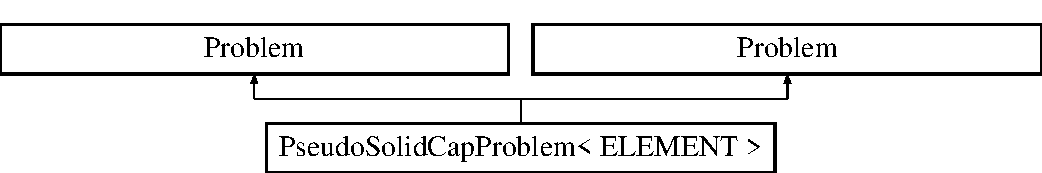
\includegraphics[height=2.000000cm]{classPseudoSolidCapProblem}
\end{center}
\end{figure}
\subsection*{Public Member Functions}
\begin{DoxyCompactItemize}
\item 
\hyperlink{classPseudoSolidCapProblem_a4ac05a07dd55950bb67f7f79cb9fbb77}{Pseudo\+Solid\+Cap\+Problem} (const bool \&hijack\+\_\+internal)
\item 
\hyperlink{classPseudoSolidCapProblem_aec2a79e44dfd785b2978419210b053b8}{$\sim$\+Pseudo\+Solid\+Cap\+Problem} ()
\begin{DoxyCompactList}\small\item\em Destructor\+: clean up memory allocated by the object. \end{DoxyCompactList}\item 
void \hyperlink{classPseudoSolidCapProblem_ae86ecaf62fa0920f5d14bf82a7f83b0e}{parameter\+\_\+study} (const string \&dir\+\_\+name)
\item 
void \hyperlink{classPseudoSolidCapProblem_a2fb98a37bde5742cbdf3c91cb1f5eb2f}{doc\+\_\+solution} (Doc\+Info \&doc\+\_\+info)
\begin{DoxyCompactList}\small\item\em Doc the solution. \end{DoxyCompactList}\item 
\hyperlink{classPseudoSolidCapProblem_a4e8963d64b50a96902169838cc195903}{Pseudo\+Solid\+Cap\+Problem} (const unsigned \&Nx, const unsigned \&Nh1, const unsigned \&Nh2)
\item 
\hyperlink{classPseudoSolidCapProblem_aec2a79e44dfd785b2978419210b053b8}{$\sim$\+Pseudo\+Solid\+Cap\+Problem} ()
\begin{DoxyCompactList}\small\item\em Destructor\+: clean up memory allocated by the object. \end{DoxyCompactList}\item 
void \hyperlink{classPseudoSolidCapProblem_ae86ecaf62fa0920f5d14bf82a7f83b0e}{parameter\+\_\+study} (const string \&dir\+\_\+name)
\item 
void \hyperlink{classPseudoSolidCapProblem_a2fb98a37bde5742cbdf3c91cb1f5eb2f}{doc\+\_\+solution} (Doc\+Info \&doc\+\_\+info)
\begin{DoxyCompactList}\small\item\em Doc the solution. \end{DoxyCompactList}\end{DoxyCompactItemize}
\subsection*{Private Member Functions}
\begin{DoxyCompactItemize}
\item 
void \hyperlink{classPseudoSolidCapProblem_ac0219ed64385dc20c4fc3c6cc217fd67}{create\+\_\+free\+\_\+surface\+\_\+elements} ()
\begin{DoxyCompactList}\small\item\em Create the free surface elements. \end{DoxyCompactList}\item 
void \hyperlink{classPseudoSolidCapProblem_a0289801610e2bc864c67d4d8557d56b1}{create\+\_\+volume\+\_\+constraint\+\_\+elements} ()
\begin{DoxyCompactList}\small\item\em Create the volume constraint elements. \end{DoxyCompactList}\item 
void \hyperlink{classPseudoSolidCapProblem_a8f28ebf09bc66142725139291b4e21a0}{create\+\_\+contact\+\_\+angle\+\_\+element} ()
\begin{DoxyCompactList}\small\item\em Create the contact angle element. \end{DoxyCompactList}\item 
void \hyperlink{classPseudoSolidCapProblem_ac0219ed64385dc20c4fc3c6cc217fd67}{create\+\_\+free\+\_\+surface\+\_\+elements} ()
\begin{DoxyCompactList}\small\item\em Create the free surface elements. \end{DoxyCompactList}\item 
void \hyperlink{classPseudoSolidCapProblem_a0289801610e2bc864c67d4d8557d56b1}{create\+\_\+volume\+\_\+constraint\+\_\+elements} ()
\begin{DoxyCompactList}\small\item\em Create the volume constraint elements. \end{DoxyCompactList}\item 
void \hyperlink{classPseudoSolidCapProblem_a8f28ebf09bc66142725139291b4e21a0}{create\+\_\+contact\+\_\+angle\+\_\+element} ()
\begin{DoxyCompactList}\small\item\em Create the contact angle element. \end{DoxyCompactList}\end{DoxyCompactItemize}
\subsection*{Private Attributes}
\begin{DoxyCompactItemize}
\item 
double \hyperlink{classPseudoSolidCapProblem_ad29a43062d88106c495d407abeddd88d}{Ca}
\begin{DoxyCompactList}\small\item\em The Capillary number. \end{DoxyCompactList}\item 
double \hyperlink{classPseudoSolidCapProblem_a49945d8e5740977a72c63e333a65293f}{Volume}
\begin{DoxyCompactList}\small\item\em The prescribed volume of the fluid. \end{DoxyCompactList}\item 
double \hyperlink{classPseudoSolidCapProblem_afbcfe3a5a05d191c44815681e4b621d0}{Pext}
\begin{DoxyCompactList}\small\item\em The external pressure. \end{DoxyCompactList}\item 
double \hyperlink{classPseudoSolidCapProblem_a51dfbd14a2cca78dc0efe6740337a22b}{Angle}
\begin{DoxyCompactList}\small\item\em The contact angle. \end{DoxyCompactList}\item 
Constitutive\+Law $\ast$ \hyperlink{classPseudoSolidCapProblem_a9eb1383956f3448a8c2e163aa2db72d7}{Constitutive\+\_\+law\+\_\+pt}
\begin{DoxyCompactList}\small\item\em Constitutive law used to determine the mesh deformation. \end{DoxyCompactList}\item 
Data $\ast$ \hyperlink{classPseudoSolidCapProblem_a51ac066b9117f30679fef658ff66d981}{External\+\_\+pressure\+\_\+data\+\_\+pt}
\begin{DoxyCompactList}\small\item\em Data object whose single value stores the external pressure. \end{DoxyCompactList}\item 
Data $\ast$ \hyperlink{classPseudoSolidCapProblem_a55491b1b87f858b8d711a362f4c70838}{Traded\+\_\+pressure\+\_\+data\+\_\+pt}
\item 
ofstream \hyperlink{classPseudoSolidCapProblem_a81d2d9915ba7d9a9a691ca2f2080b6b4}{Trace\+\_\+file}
\begin{DoxyCompactList}\small\item\em Trace file. \end{DoxyCompactList}\item 
Mesh $\ast$ \hyperlink{classPseudoSolidCapProblem_a6d4520b30d05f3dde12ea9bae9d62d0b}{Bulk\+\_\+mesh\+\_\+pt}
\begin{DoxyCompactList}\small\item\em Storage for the bulk mesh. \end{DoxyCompactList}\item 
Mesh $\ast$ \hyperlink{classPseudoSolidCapProblem_ac1de72bb2e35d6fbd76ef0ea6c19dc48}{Free\+\_\+surface\+\_\+mesh\+\_\+pt}
\begin{DoxyCompactList}\small\item\em Storage for the free surface mesh. \end{DoxyCompactList}\item 
Mesh $\ast$ \hyperlink{classPseudoSolidCapProblem_ab0e178700d6f9d2b6a86ae58483d6e2e}{Free\+\_\+surface\+\_\+bounding\+\_\+mesh\+\_\+pt}
\begin{DoxyCompactList}\small\item\em Storage for the element bounding the free surface. \end{DoxyCompactList}\item 
Mesh $\ast$ \hyperlink{classPseudoSolidCapProblem_a173d08853c11d0692a4e922bc3fcf53f}{Volume\+\_\+computation\+\_\+mesh\+\_\+pt}
\begin{DoxyCompactList}\small\item\em Storage for the elements that compute the enclosed volume. \end{DoxyCompactList}\item 
Mesh $\ast$ \hyperlink{classPseudoSolidCapProblem_a65b3318c82437c510f23ee0ae898ff6c}{Volume\+\_\+constraint\+\_\+mesh\+\_\+pt}
\begin{DoxyCompactList}\small\item\em Storage for the volume constraint. \end{DoxyCompactList}\item 
\hyperlink{classElasticTwoLayerMesh}{Elastic\+Two\+Layer\+Mesh}$<$ E\+L\+E\+M\+E\+NT $>$ $\ast$ \hyperlink{classPseudoSolidCapProblem_a24ee2e5afd19ab0febf85306d45c8385}{Bulk\+\_\+mesh\+\_\+pt}
\begin{DoxyCompactList}\small\item\em Storage for the bulk mesh. \end{DoxyCompactList}\end{DoxyCompactItemize}


\subsection{Detailed Description}
\subsubsection*{template$<$class E\+L\+E\+M\+E\+NT$>$\newline
class Pseudo\+Solid\+Cap\+Problem$<$ E\+L\+E\+M\+E\+N\+T $>$}

A class that solves the Navier--Stokes equations to compute the shape of a static interface in a rectangular container with imposed contact angle at the boundary. 

A class that solves the Navier--Stokes equations to compute the shape of a static interface between two fluids in a rectangular container with an imposed contact angle at the boundary. 

Definition at line 508 of file static\+\_\+single\+\_\+layer.\+cc.



\subsection{Constructor \& Destructor Documentation}
\mbox{\Hypertarget{classPseudoSolidCapProblem_a4ac05a07dd55950bb67f7f79cb9fbb77}\label{classPseudoSolidCapProblem_a4ac05a07dd55950bb67f7f79cb9fbb77}} 
\index{Pseudo\+Solid\+Cap\+Problem@{Pseudo\+Solid\+Cap\+Problem}!Pseudo\+Solid\+Cap\+Problem@{Pseudo\+Solid\+Cap\+Problem}}
\index{Pseudo\+Solid\+Cap\+Problem@{Pseudo\+Solid\+Cap\+Problem}!Pseudo\+Solid\+Cap\+Problem@{Pseudo\+Solid\+Cap\+Problem}}
\subsubsection{\texorpdfstring{Pseudo\+Solid\+Cap\+Problem()}{PseudoSolidCapProblem()}\hspace{0.1cm}{\footnotesize\ttfamily [1/2]}}
{\footnotesize\ttfamily template$<$class E\+L\+E\+M\+E\+NT $>$ \\
\hyperlink{classPseudoSolidCapProblem}{Pseudo\+Solid\+Cap\+Problem}$<$ E\+L\+E\+M\+E\+NT $>$\+::\hyperlink{classPseudoSolidCapProblem}{Pseudo\+Solid\+Cap\+Problem} (\begin{DoxyParamCaption}\item[{const bool \&}]{hijack\+\_\+internal }\end{DoxyParamCaption})}

Constructor\+: Boolean flag indicates if volume constraint is applied by hijacking internal or external pressure

Constructor\+: Pass boolean flag to indicate if the volume constraint is applied by hijacking an internal pressure or the external pressure 

Definition at line 588 of file static\+\_\+single\+\_\+layer.\+cc.



References Pseudo\+Solid\+Cap\+Problem$<$ E\+L\+E\+M\+E\+N\+T $>$\+::\+Bulk\+\_\+mesh\+\_\+pt, Pseudo\+Solid\+Cap\+Problem$<$ E\+L\+E\+M\+E\+N\+T $>$\+::\+Constitutive\+\_\+law\+\_\+pt, Pseudo\+Solid\+Cap\+Problem$<$ E\+L\+E\+M\+E\+N\+T $>$\+::create\+\_\+contact\+\_\+angle\+\_\+element(), Pseudo\+Solid\+Cap\+Problem$<$ E\+L\+E\+M\+E\+N\+T $>$\+::create\+\_\+free\+\_\+surface\+\_\+elements(), Pseudo\+Solid\+Cap\+Problem$<$ E\+L\+E\+M\+E\+N\+T $>$\+::create\+\_\+volume\+\_\+constraint\+\_\+elements(), Pseudo\+Solid\+Cap\+Problem$<$ E\+L\+E\+M\+E\+N\+T $>$\+::\+External\+\_\+pressure\+\_\+data\+\_\+pt, Pseudo\+Solid\+Cap\+Problem$<$ E\+L\+E\+M\+E\+N\+T $>$\+::\+Free\+\_\+surface\+\_\+bounding\+\_\+mesh\+\_\+pt, Pseudo\+Solid\+Cap\+Problem$<$ E\+L\+E\+M\+E\+N\+T $>$\+::\+Free\+\_\+surface\+\_\+mesh\+\_\+pt, Global\+\_\+\+Physical\+\_\+\+Variables\+::\+Nu, Pseudo\+Solid\+Cap\+Problem$<$ E\+L\+E\+M\+E\+N\+T $>$\+::\+Pext, Pseudo\+Solid\+Cap\+Problem$<$ E\+L\+E\+M\+E\+N\+T $>$\+::\+Traded\+\_\+pressure\+\_\+data\+\_\+pt, Pseudo\+Solid\+Cap\+Problem$<$ E\+L\+E\+M\+E\+N\+T $>$\+::\+Volume\+\_\+computation\+\_\+mesh\+\_\+pt, Pseudo\+Solid\+Cap\+Problem$<$ E\+L\+E\+M\+E\+N\+T $>$\+::\+Volume\+\_\+constraint\+\_\+mesh\+\_\+pt, and Global\+\_\+\+Physical\+\_\+\+Variables\+::\+Wall\+\_\+normal.

\mbox{\Hypertarget{classPseudoSolidCapProblem_aec2a79e44dfd785b2978419210b053b8}\label{classPseudoSolidCapProblem_aec2a79e44dfd785b2978419210b053b8}} 
\index{Pseudo\+Solid\+Cap\+Problem@{Pseudo\+Solid\+Cap\+Problem}!````~Pseudo\+Solid\+Cap\+Problem@{$\sim$\+Pseudo\+Solid\+Cap\+Problem}}
\index{````~Pseudo\+Solid\+Cap\+Problem@{$\sim$\+Pseudo\+Solid\+Cap\+Problem}!Pseudo\+Solid\+Cap\+Problem@{Pseudo\+Solid\+Cap\+Problem}}
\subsubsection{\texorpdfstring{$\sim$\+Pseudo\+Solid\+Cap\+Problem()}{~PseudoSolidCapProblem()}\hspace{0.1cm}{\footnotesize\ttfamily [1/2]}}
{\footnotesize\ttfamily template$<$class E\+L\+E\+M\+E\+NT $>$ \\
\hyperlink{classPseudoSolidCapProblem}{Pseudo\+Solid\+Cap\+Problem}$<$ E\+L\+E\+M\+E\+NT $>$\+::$\sim$\hyperlink{classPseudoSolidCapProblem}{Pseudo\+Solid\+Cap\+Problem} (\begin{DoxyParamCaption}{ }\end{DoxyParamCaption})}



Destructor\+: clean up memory allocated by the object. 

Destructor. Make sure to clean up all allocated memory, so that multiple instances of the problem don\textquotesingle{}t lead to excessive memory usage. 

Definition at line 758 of file static\+\_\+single\+\_\+layer.\+cc.



References Pseudo\+Solid\+Cap\+Problem$<$ E\+L\+E\+M\+E\+N\+T $>$\+::\+Bulk\+\_\+mesh\+\_\+pt, Pseudo\+Solid\+Cap\+Problem$<$ E\+L\+E\+M\+E\+N\+T $>$\+::\+Constitutive\+\_\+law\+\_\+pt, Pseudo\+Solid\+Cap\+Problem$<$ E\+L\+E\+M\+E\+N\+T $>$\+::\+External\+\_\+pressure\+\_\+data\+\_\+pt, Pseudo\+Solid\+Cap\+Problem$<$ E\+L\+E\+M\+E\+N\+T $>$\+::\+Free\+\_\+surface\+\_\+bounding\+\_\+mesh\+\_\+pt, Pseudo\+Solid\+Cap\+Problem$<$ E\+L\+E\+M\+E\+N\+T $>$\+::\+Free\+\_\+surface\+\_\+mesh\+\_\+pt, Pseudo\+Solid\+Cap\+Problem$<$ E\+L\+E\+M\+E\+N\+T $>$\+::\+Traded\+\_\+pressure\+\_\+data\+\_\+pt, Pseudo\+Solid\+Cap\+Problem$<$ E\+L\+E\+M\+E\+N\+T $>$\+::\+Volume\+\_\+computation\+\_\+mesh\+\_\+pt, and Pseudo\+Solid\+Cap\+Problem$<$ E\+L\+E\+M\+E\+N\+T $>$\+::\+Volume\+\_\+constraint\+\_\+mesh\+\_\+pt.



Referenced by Pseudo\+Solid\+Cap\+Problem$<$ E\+L\+E\+M\+E\+N\+T $>$\+::\+Pseudo\+Solid\+Cap\+Problem().

\mbox{\Hypertarget{classPseudoSolidCapProblem_a4e8963d64b50a96902169838cc195903}\label{classPseudoSolidCapProblem_a4e8963d64b50a96902169838cc195903}} 
\index{Pseudo\+Solid\+Cap\+Problem@{Pseudo\+Solid\+Cap\+Problem}!Pseudo\+Solid\+Cap\+Problem@{Pseudo\+Solid\+Cap\+Problem}}
\index{Pseudo\+Solid\+Cap\+Problem@{Pseudo\+Solid\+Cap\+Problem}!Pseudo\+Solid\+Cap\+Problem@{Pseudo\+Solid\+Cap\+Problem}}
\subsubsection{\texorpdfstring{Pseudo\+Solid\+Cap\+Problem()}{PseudoSolidCapProblem()}\hspace{0.1cm}{\footnotesize\ttfamily [2/2]}}
{\footnotesize\ttfamily template$<$class E\+L\+E\+M\+E\+NT $>$ \\
\hyperlink{classPseudoSolidCapProblem}{Pseudo\+Solid\+Cap\+Problem}$<$ E\+L\+E\+M\+E\+NT $>$\+::\hyperlink{classPseudoSolidCapProblem}{Pseudo\+Solid\+Cap\+Problem} (\begin{DoxyParamCaption}\item[{const unsigned \&}]{Nx,  }\item[{const unsigned \&}]{Nh1,  }\item[{const unsigned \&}]{Nh2 }\end{DoxyParamCaption})}

Constructor\+: Pass boolean flag to indicate if the volume constraint is applied by hijacking an internal pressure or the external pressure 

Definition at line 832 of file static\+\_\+two\+\_\+layer.\+cc.



References Pseudo\+Solid\+Cap\+Problem$<$ E\+L\+E\+M\+E\+N\+T $>$\+::\+Angle, Pseudo\+Solid\+Cap\+Problem$<$ E\+L\+E\+M\+E\+N\+T $>$\+::\+Bulk\+\_\+mesh\+\_\+pt, Pseudo\+Solid\+Cap\+Problem$<$ E\+L\+E\+M\+E\+N\+T $>$\+::\+Ca, Pseudo\+Solid\+Cap\+Problem$<$ E\+L\+E\+M\+E\+N\+T $>$\+::\+Constitutive\+\_\+law\+\_\+pt, Pseudo\+Solid\+Cap\+Problem$<$ E\+L\+E\+M\+E\+N\+T $>$\+::create\+\_\+contact\+\_\+angle\+\_\+element(), Pseudo\+Solid\+Cap\+Problem$<$ E\+L\+E\+M\+E\+N\+T $>$\+::create\+\_\+free\+\_\+surface\+\_\+elements(), Pseudo\+Solid\+Cap\+Problem$<$ E\+L\+E\+M\+E\+N\+T $>$\+::create\+\_\+volume\+\_\+constraint\+\_\+elements(), Pseudo\+Solid\+Cap\+Problem$<$ E\+L\+E\+M\+E\+N\+T $>$\+::doc\+\_\+solution(), Pseudo\+Solid\+Cap\+Problem$<$ E\+L\+E\+M\+E\+N\+T $>$\+::\+Free\+\_\+surface\+\_\+bounding\+\_\+mesh\+\_\+pt, Pseudo\+Solid\+Cap\+Problem$<$ E\+L\+E\+M\+E\+N\+T $>$\+::\+Free\+\_\+surface\+\_\+mesh\+\_\+pt, Global\+\_\+\+Physical\+\_\+\+Variables\+::\+Nu, Pseudo\+Solid\+Cap\+Problem$<$ E\+L\+E\+M\+E\+N\+T $>$\+::parameter\+\_\+study(), Pseudo\+Solid\+Cap\+Problem$<$ E\+L\+E\+M\+E\+N\+T $>$\+::\+Trace\+\_\+file, Pseudo\+Solid\+Cap\+Problem$<$ E\+L\+E\+M\+E\+N\+T $>$\+::\+Traded\+\_\+pressure\+\_\+data\+\_\+pt, Pseudo\+Solid\+Cap\+Problem$<$ E\+L\+E\+M\+E\+N\+T $>$\+::\+Volume, Pseudo\+Solid\+Cap\+Problem$<$ E\+L\+E\+M\+E\+N\+T $>$\+::\+Volume\+\_\+computation\+\_\+mesh\+\_\+pt, Pseudo\+Solid\+Cap\+Problem$<$ E\+L\+E\+M\+E\+N\+T $>$\+::\+Volume\+\_\+constraint\+\_\+mesh\+\_\+pt, Global\+\_\+\+Physical\+\_\+\+Variables\+::\+Wall\+\_\+normal, Global\+\_\+\+Physical\+\_\+\+Variables\+::wall\+\_\+unit\+\_\+normal\+\_\+fct(), and Pseudo\+Solid\+Cap\+Problem$<$ E\+L\+E\+M\+E\+N\+T $>$\+::$\sim$\+Pseudo\+Solid\+Cap\+Problem().

\mbox{\Hypertarget{classPseudoSolidCapProblem_aec2a79e44dfd785b2978419210b053b8}\label{classPseudoSolidCapProblem_aec2a79e44dfd785b2978419210b053b8}} 
\index{Pseudo\+Solid\+Cap\+Problem@{Pseudo\+Solid\+Cap\+Problem}!````~Pseudo\+Solid\+Cap\+Problem@{$\sim$\+Pseudo\+Solid\+Cap\+Problem}}
\index{````~Pseudo\+Solid\+Cap\+Problem@{$\sim$\+Pseudo\+Solid\+Cap\+Problem}!Pseudo\+Solid\+Cap\+Problem@{Pseudo\+Solid\+Cap\+Problem}}
\subsubsection{\texorpdfstring{$\sim$\+Pseudo\+Solid\+Cap\+Problem()}{~PseudoSolidCapProblem()}\hspace{0.1cm}{\footnotesize\ttfamily [2/2]}}
{\footnotesize\ttfamily template$<$class E\+L\+E\+M\+E\+NT $>$ \\
\hyperlink{classPseudoSolidCapProblem}{Pseudo\+Solid\+Cap\+Problem}$<$ E\+L\+E\+M\+E\+NT $>$\+::$\sim$\hyperlink{classPseudoSolidCapProblem}{Pseudo\+Solid\+Cap\+Problem} (\begin{DoxyParamCaption}{ }\end{DoxyParamCaption})}



Destructor\+: clean up memory allocated by the object. 



\subsection{Member Function Documentation}
\mbox{\Hypertarget{classPseudoSolidCapProblem_a8f28ebf09bc66142725139291b4e21a0}\label{classPseudoSolidCapProblem_a8f28ebf09bc66142725139291b4e21a0}} 
\index{Pseudo\+Solid\+Cap\+Problem@{Pseudo\+Solid\+Cap\+Problem}!create\+\_\+contact\+\_\+angle\+\_\+element@{create\+\_\+contact\+\_\+angle\+\_\+element}}
\index{create\+\_\+contact\+\_\+angle\+\_\+element@{create\+\_\+contact\+\_\+angle\+\_\+element}!Pseudo\+Solid\+Cap\+Problem@{Pseudo\+Solid\+Cap\+Problem}}
\subsubsection{\texorpdfstring{create\+\_\+contact\+\_\+angle\+\_\+element()}{create\_contact\_angle\_element()}\hspace{0.1cm}{\footnotesize\ttfamily [1/2]}}
{\footnotesize\ttfamily template$<$class E\+L\+E\+M\+E\+NT $>$ \\
void \hyperlink{classPseudoSolidCapProblem}{Pseudo\+Solid\+Cap\+Problem}$<$ E\+L\+E\+M\+E\+NT $>$\+::create\+\_\+contact\+\_\+angle\+\_\+element (\begin{DoxyParamCaption}{ }\end{DoxyParamCaption})\hspace{0.3cm}{\ttfamily [private]}}



Create the contact angle element. 



Definition at line 892 of file static\+\_\+single\+\_\+layer.\+cc.



References Pseudo\+Solid\+Cap\+Problem$<$ E\+L\+E\+M\+E\+N\+T $>$\+::\+Angle, Pseudo\+Solid\+Cap\+Problem$<$ E\+L\+E\+M\+E\+N\+T $>$\+::\+Ca, Pseudo\+Solid\+Cap\+Problem$<$ E\+L\+E\+M\+E\+N\+T $>$\+::\+Free\+\_\+surface\+\_\+bounding\+\_\+mesh\+\_\+pt, Pseudo\+Solid\+Cap\+Problem$<$ E\+L\+E\+M\+E\+N\+T $>$\+::\+Free\+\_\+surface\+\_\+mesh\+\_\+pt, and Global\+\_\+\+Physical\+\_\+\+Variables\+::wall\+\_\+unit\+\_\+normal\+\_\+fct().



Referenced by Pseudo\+Solid\+Cap\+Problem$<$ E\+L\+E\+M\+E\+N\+T $>$\+::\+Pseudo\+Solid\+Cap\+Problem().

\mbox{\Hypertarget{classPseudoSolidCapProblem_a8f28ebf09bc66142725139291b4e21a0}\label{classPseudoSolidCapProblem_a8f28ebf09bc66142725139291b4e21a0}} 
\index{Pseudo\+Solid\+Cap\+Problem@{Pseudo\+Solid\+Cap\+Problem}!create\+\_\+contact\+\_\+angle\+\_\+element@{create\+\_\+contact\+\_\+angle\+\_\+element}}
\index{create\+\_\+contact\+\_\+angle\+\_\+element@{create\+\_\+contact\+\_\+angle\+\_\+element}!Pseudo\+Solid\+Cap\+Problem@{Pseudo\+Solid\+Cap\+Problem}}
\subsubsection{\texorpdfstring{create\+\_\+contact\+\_\+angle\+\_\+element()}{create\_contact\_angle\_element()}\hspace{0.1cm}{\footnotesize\ttfamily [2/2]}}
{\footnotesize\ttfamily template$<$class E\+L\+E\+M\+E\+NT $>$ \\
void \hyperlink{classPseudoSolidCapProblem}{Pseudo\+Solid\+Cap\+Problem}$<$ E\+L\+E\+M\+E\+NT $>$\+::create\+\_\+contact\+\_\+angle\+\_\+element (\begin{DoxyParamCaption}{ }\end{DoxyParamCaption})\hspace{0.3cm}{\ttfamily [private]}}



Create the contact angle element. 

\mbox{\Hypertarget{classPseudoSolidCapProblem_ac0219ed64385dc20c4fc3c6cc217fd67}\label{classPseudoSolidCapProblem_ac0219ed64385dc20c4fc3c6cc217fd67}} 
\index{Pseudo\+Solid\+Cap\+Problem@{Pseudo\+Solid\+Cap\+Problem}!create\+\_\+free\+\_\+surface\+\_\+elements@{create\+\_\+free\+\_\+surface\+\_\+elements}}
\index{create\+\_\+free\+\_\+surface\+\_\+elements@{create\+\_\+free\+\_\+surface\+\_\+elements}!Pseudo\+Solid\+Cap\+Problem@{Pseudo\+Solid\+Cap\+Problem}}
\subsubsection{\texorpdfstring{create\+\_\+free\+\_\+surface\+\_\+elements()}{create\_free\_surface\_elements()}\hspace{0.1cm}{\footnotesize\ttfamily [1/2]}}
{\footnotesize\ttfamily template$<$class E\+L\+E\+M\+E\+NT $>$ \\
void \hyperlink{classPseudoSolidCapProblem}{Pseudo\+Solid\+Cap\+Problem}$<$ E\+L\+E\+M\+E\+NT $>$\+::create\+\_\+free\+\_\+surface\+\_\+elements (\begin{DoxyParamCaption}{ }\end{DoxyParamCaption})\hspace{0.3cm}{\ttfamily [private]}}



Create the free surface elements. 



Definition at line 799 of file static\+\_\+single\+\_\+layer.\+cc.



References Pseudo\+Solid\+Cap\+Problem$<$ E\+L\+E\+M\+E\+N\+T $>$\+::\+Bulk\+\_\+mesh\+\_\+pt, Pseudo\+Solid\+Cap\+Problem$<$ E\+L\+E\+M\+E\+N\+T $>$\+::\+Ca, Pseudo\+Solid\+Cap\+Problem$<$ E\+L\+E\+M\+E\+N\+T $>$\+::\+External\+\_\+pressure\+\_\+data\+\_\+pt, and Pseudo\+Solid\+Cap\+Problem$<$ E\+L\+E\+M\+E\+N\+T $>$\+::\+Free\+\_\+surface\+\_\+mesh\+\_\+pt.



Referenced by Pseudo\+Solid\+Cap\+Problem$<$ E\+L\+E\+M\+E\+N\+T $>$\+::\+Pseudo\+Solid\+Cap\+Problem().

\mbox{\Hypertarget{classPseudoSolidCapProblem_ac0219ed64385dc20c4fc3c6cc217fd67}\label{classPseudoSolidCapProblem_ac0219ed64385dc20c4fc3c6cc217fd67}} 
\index{Pseudo\+Solid\+Cap\+Problem@{Pseudo\+Solid\+Cap\+Problem}!create\+\_\+free\+\_\+surface\+\_\+elements@{create\+\_\+free\+\_\+surface\+\_\+elements}}
\index{create\+\_\+free\+\_\+surface\+\_\+elements@{create\+\_\+free\+\_\+surface\+\_\+elements}!Pseudo\+Solid\+Cap\+Problem@{Pseudo\+Solid\+Cap\+Problem}}
\subsubsection{\texorpdfstring{create\+\_\+free\+\_\+surface\+\_\+elements()}{create\_free\_surface\_elements()}\hspace{0.1cm}{\footnotesize\ttfamily [2/2]}}
{\footnotesize\ttfamily template$<$class E\+L\+E\+M\+E\+NT $>$ \\
void \hyperlink{classPseudoSolidCapProblem}{Pseudo\+Solid\+Cap\+Problem}$<$ E\+L\+E\+M\+E\+NT $>$\+::create\+\_\+free\+\_\+surface\+\_\+elements (\begin{DoxyParamCaption}{ }\end{DoxyParamCaption})\hspace{0.3cm}{\ttfamily [private]}}



Create the free surface elements. 

\mbox{\Hypertarget{classPseudoSolidCapProblem_a0289801610e2bc864c67d4d8557d56b1}\label{classPseudoSolidCapProblem_a0289801610e2bc864c67d4d8557d56b1}} 
\index{Pseudo\+Solid\+Cap\+Problem@{Pseudo\+Solid\+Cap\+Problem}!create\+\_\+volume\+\_\+constraint\+\_\+elements@{create\+\_\+volume\+\_\+constraint\+\_\+elements}}
\index{create\+\_\+volume\+\_\+constraint\+\_\+elements@{create\+\_\+volume\+\_\+constraint\+\_\+elements}!Pseudo\+Solid\+Cap\+Problem@{Pseudo\+Solid\+Cap\+Problem}}
\subsubsection{\texorpdfstring{create\+\_\+volume\+\_\+constraint\+\_\+elements()}{create\_volume\_constraint\_elements()}\hspace{0.1cm}{\footnotesize\ttfamily [1/2]}}
{\footnotesize\ttfamily template$<$class E\+L\+E\+M\+E\+NT $>$ \\
void \hyperlink{classPseudoSolidCapProblem}{Pseudo\+Solid\+Cap\+Problem}$<$ E\+L\+E\+M\+E\+NT $>$\+::create\+\_\+volume\+\_\+constraint\+\_\+elements (\begin{DoxyParamCaption}{ }\end{DoxyParamCaption})\hspace{0.3cm}{\ttfamily [private]}}



Create the volume constraint elements. 



Definition at line 846 of file static\+\_\+single\+\_\+layer.\+cc.



References Pseudo\+Solid\+Cap\+Problem$<$ E\+L\+E\+M\+E\+N\+T $>$\+::\+Bulk\+\_\+mesh\+\_\+pt, Pseudo\+Solid\+Cap\+Problem$<$ E\+L\+E\+M\+E\+N\+T $>$\+::\+Traded\+\_\+pressure\+\_\+data\+\_\+pt, Pseudo\+Solid\+Cap\+Problem$<$ E\+L\+E\+M\+E\+N\+T $>$\+::\+Volume, Pseudo\+Solid\+Cap\+Problem$<$ E\+L\+E\+M\+E\+N\+T $>$\+::\+Volume\+\_\+computation\+\_\+mesh\+\_\+pt, and Pseudo\+Solid\+Cap\+Problem$<$ E\+L\+E\+M\+E\+N\+T $>$\+::\+Volume\+\_\+constraint\+\_\+mesh\+\_\+pt.



Referenced by Pseudo\+Solid\+Cap\+Problem$<$ E\+L\+E\+M\+E\+N\+T $>$\+::\+Pseudo\+Solid\+Cap\+Problem().

\mbox{\Hypertarget{classPseudoSolidCapProblem_a0289801610e2bc864c67d4d8557d56b1}\label{classPseudoSolidCapProblem_a0289801610e2bc864c67d4d8557d56b1}} 
\index{Pseudo\+Solid\+Cap\+Problem@{Pseudo\+Solid\+Cap\+Problem}!create\+\_\+volume\+\_\+constraint\+\_\+elements@{create\+\_\+volume\+\_\+constraint\+\_\+elements}}
\index{create\+\_\+volume\+\_\+constraint\+\_\+elements@{create\+\_\+volume\+\_\+constraint\+\_\+elements}!Pseudo\+Solid\+Cap\+Problem@{Pseudo\+Solid\+Cap\+Problem}}
\subsubsection{\texorpdfstring{create\+\_\+volume\+\_\+constraint\+\_\+elements()}{create\_volume\_constraint\_elements()}\hspace{0.1cm}{\footnotesize\ttfamily [2/2]}}
{\footnotesize\ttfamily template$<$class E\+L\+E\+M\+E\+NT $>$ \\
void \hyperlink{classPseudoSolidCapProblem}{Pseudo\+Solid\+Cap\+Problem}$<$ E\+L\+E\+M\+E\+NT $>$\+::create\+\_\+volume\+\_\+constraint\+\_\+elements (\begin{DoxyParamCaption}{ }\end{DoxyParamCaption})\hspace{0.3cm}{\ttfamily [private]}}



Create the volume constraint elements. 

\mbox{\Hypertarget{classPseudoSolidCapProblem_a2fb98a37bde5742cbdf3c91cb1f5eb2f}\label{classPseudoSolidCapProblem_a2fb98a37bde5742cbdf3c91cb1f5eb2f}} 
\index{Pseudo\+Solid\+Cap\+Problem@{Pseudo\+Solid\+Cap\+Problem}!doc\+\_\+solution@{doc\+\_\+solution}}
\index{doc\+\_\+solution@{doc\+\_\+solution}!Pseudo\+Solid\+Cap\+Problem@{Pseudo\+Solid\+Cap\+Problem}}
\subsubsection{\texorpdfstring{doc\+\_\+solution()}{doc\_solution()}\hspace{0.1cm}{\footnotesize\ttfamily [1/2]}}
{\footnotesize\ttfamily template$<$class E\+L\+E\+M\+E\+NT $>$ \\
void \hyperlink{classPseudoSolidCapProblem}{Pseudo\+Solid\+Cap\+Problem}$<$ E\+L\+E\+M\+E\+NT $>$\+::doc\+\_\+solution (\begin{DoxyParamCaption}\item[{Doc\+Info \&}]{doc\+\_\+info }\end{DoxyParamCaption})}



Doc the solution. 



Definition at line 971 of file static\+\_\+single\+\_\+layer.\+cc.



References Pseudo\+Solid\+Cap\+Problem$<$ E\+L\+E\+M\+E\+N\+T $>$\+::\+Angle, Pseudo\+Solid\+Cap\+Problem$<$ E\+L\+E\+M\+E\+N\+T $>$\+::\+Bulk\+\_\+mesh\+\_\+pt, Pseudo\+Solid\+Cap\+Problem$<$ E\+L\+E\+M\+E\+N\+T $>$\+::\+Ca, Pseudo\+Solid\+Cap\+Problem$<$ E\+L\+E\+M\+E\+N\+T $>$\+::\+External\+\_\+pressure\+\_\+data\+\_\+pt, Pseudo\+Solid\+Cap\+Problem$<$ E\+L\+E\+M\+E\+N\+T $>$\+::\+Free\+\_\+surface\+\_\+mesh\+\_\+pt, and Pseudo\+Solid\+Cap\+Problem$<$ E\+L\+E\+M\+E\+N\+T $>$\+::\+Trace\+\_\+file.



Referenced by Pseudo\+Solid\+Cap\+Problem$<$ E\+L\+E\+M\+E\+N\+T $>$\+::parameter\+\_\+study(), and Pseudo\+Solid\+Cap\+Problem$<$ E\+L\+E\+M\+E\+N\+T $>$\+::\+Pseudo\+Solid\+Cap\+Problem().

\mbox{\Hypertarget{classPseudoSolidCapProblem_a2fb98a37bde5742cbdf3c91cb1f5eb2f}\label{classPseudoSolidCapProblem_a2fb98a37bde5742cbdf3c91cb1f5eb2f}} 
\index{Pseudo\+Solid\+Cap\+Problem@{Pseudo\+Solid\+Cap\+Problem}!doc\+\_\+solution@{doc\+\_\+solution}}
\index{doc\+\_\+solution@{doc\+\_\+solution}!Pseudo\+Solid\+Cap\+Problem@{Pseudo\+Solid\+Cap\+Problem}}
\subsubsection{\texorpdfstring{doc\+\_\+solution()}{doc\_solution()}\hspace{0.1cm}{\footnotesize\ttfamily [2/2]}}
{\footnotesize\ttfamily template$<$class E\+L\+E\+M\+E\+NT $>$ \\
void \hyperlink{classPseudoSolidCapProblem}{Pseudo\+Solid\+Cap\+Problem}$<$ E\+L\+E\+M\+E\+NT $>$\+::doc\+\_\+solution (\begin{DoxyParamCaption}\item[{Doc\+Info \&}]{doc\+\_\+info }\end{DoxyParamCaption})}



Doc the solution. 

\mbox{\Hypertarget{classPseudoSolidCapProblem_ae86ecaf62fa0920f5d14bf82a7f83b0e}\label{classPseudoSolidCapProblem_ae86ecaf62fa0920f5d14bf82a7f83b0e}} 
\index{Pseudo\+Solid\+Cap\+Problem@{Pseudo\+Solid\+Cap\+Problem}!parameter\+\_\+study@{parameter\+\_\+study}}
\index{parameter\+\_\+study@{parameter\+\_\+study}!Pseudo\+Solid\+Cap\+Problem@{Pseudo\+Solid\+Cap\+Problem}}
\subsubsection{\texorpdfstring{parameter\+\_\+study()}{parameter\_study()}\hspace{0.1cm}{\footnotesize\ttfamily [1/2]}}
{\footnotesize\ttfamily template$<$class E\+L\+E\+M\+E\+NT $>$ \\
void \hyperlink{classPseudoSolidCapProblem}{Pseudo\+Solid\+Cap\+Problem}$<$ E\+L\+E\+M\+E\+NT $>$\+::parameter\+\_\+study (\begin{DoxyParamCaption}\item[{const string \&}]{dir\+\_\+name }\end{DoxyParamCaption})}

Peform a parameter study\+: Solve problem for a range of contact angles Pass name of output directory as a string

Perform a parameter study. Pass name of output directory as a string 

Definition at line 929 of file static\+\_\+single\+\_\+layer.\+cc.



References Pseudo\+Solid\+Cap\+Problem$<$ E\+L\+E\+M\+E\+N\+T $>$\+::\+Angle, Pseudo\+Solid\+Cap\+Problem$<$ E\+L\+E\+M\+E\+N\+T $>$\+::doc\+\_\+solution(), and Pseudo\+Solid\+Cap\+Problem$<$ E\+L\+E\+M\+E\+N\+T $>$\+::\+Trace\+\_\+file.



Referenced by Pseudo\+Solid\+Cap\+Problem$<$ E\+L\+E\+M\+E\+N\+T $>$\+::\+Pseudo\+Solid\+Cap\+Problem().

\mbox{\Hypertarget{classPseudoSolidCapProblem_ae86ecaf62fa0920f5d14bf82a7f83b0e}\label{classPseudoSolidCapProblem_ae86ecaf62fa0920f5d14bf82a7f83b0e}} 
\index{Pseudo\+Solid\+Cap\+Problem@{Pseudo\+Solid\+Cap\+Problem}!parameter\+\_\+study@{parameter\+\_\+study}}
\index{parameter\+\_\+study@{parameter\+\_\+study}!Pseudo\+Solid\+Cap\+Problem@{Pseudo\+Solid\+Cap\+Problem}}
\subsubsection{\texorpdfstring{parameter\+\_\+study()}{parameter\_study()}\hspace{0.1cm}{\footnotesize\ttfamily [2/2]}}
{\footnotesize\ttfamily template$<$class E\+L\+E\+M\+E\+NT $>$ \\
void \hyperlink{classPseudoSolidCapProblem}{Pseudo\+Solid\+Cap\+Problem}$<$ E\+L\+E\+M\+E\+NT $>$\+::parameter\+\_\+study (\begin{DoxyParamCaption}\item[{const string \&}]{dir\+\_\+name }\end{DoxyParamCaption})}

Peform a parameter study\+: Solve problem for a range of contact angles Pass name of output directory as a string 

\subsection{Member Data Documentation}
\mbox{\Hypertarget{classPseudoSolidCapProblem_a51dfbd14a2cca78dc0efe6740337a22b}\label{classPseudoSolidCapProblem_a51dfbd14a2cca78dc0efe6740337a22b}} 
\index{Pseudo\+Solid\+Cap\+Problem@{Pseudo\+Solid\+Cap\+Problem}!Angle@{Angle}}
\index{Angle@{Angle}!Pseudo\+Solid\+Cap\+Problem@{Pseudo\+Solid\+Cap\+Problem}}
\subsubsection{\texorpdfstring{Angle}{Angle}}
{\footnotesize\ttfamily template$<$class E\+L\+E\+M\+E\+NT $>$ \\
double \hyperlink{classPseudoSolidCapProblem}{Pseudo\+Solid\+Cap\+Problem}$<$ E\+L\+E\+M\+E\+NT $>$\+::Angle\hspace{0.3cm}{\ttfamily [private]}}



The contact angle. 



Definition at line 547 of file static\+\_\+single\+\_\+layer.\+cc.



Referenced by Pseudo\+Solid\+Cap\+Problem$<$ E\+L\+E\+M\+E\+N\+T $>$\+::create\+\_\+contact\+\_\+angle\+\_\+element(), Pseudo\+Solid\+Cap\+Problem$<$ E\+L\+E\+M\+E\+N\+T $>$\+::doc\+\_\+solution(), Pseudo\+Solid\+Cap\+Problem$<$ E\+L\+E\+M\+E\+N\+T $>$\+::parameter\+\_\+study(), and Pseudo\+Solid\+Cap\+Problem$<$ E\+L\+E\+M\+E\+N\+T $>$\+::\+Pseudo\+Solid\+Cap\+Problem().

\mbox{\Hypertarget{classPseudoSolidCapProblem_a6d4520b30d05f3dde12ea9bae9d62d0b}\label{classPseudoSolidCapProblem_a6d4520b30d05f3dde12ea9bae9d62d0b}} 
\index{Pseudo\+Solid\+Cap\+Problem@{Pseudo\+Solid\+Cap\+Problem}!Bulk\+\_\+mesh\+\_\+pt@{Bulk\+\_\+mesh\+\_\+pt}}
\index{Bulk\+\_\+mesh\+\_\+pt@{Bulk\+\_\+mesh\+\_\+pt}!Pseudo\+Solid\+Cap\+Problem@{Pseudo\+Solid\+Cap\+Problem}}
\subsubsection{\texorpdfstring{Bulk\+\_\+mesh\+\_\+pt}{Bulk\_mesh\_pt}\hspace{0.1cm}{\footnotesize\ttfamily [1/2]}}
{\footnotesize\ttfamily template$<$class E\+L\+E\+M\+E\+NT $>$ \\
Mesh$\ast$ \hyperlink{classPseudoSolidCapProblem}{Pseudo\+Solid\+Cap\+Problem}$<$ E\+L\+E\+M\+E\+NT $>$\+::Bulk\+\_\+mesh\+\_\+pt\hspace{0.3cm}{\ttfamily [private]}}



Storage for the bulk mesh. 



Definition at line 564 of file static\+\_\+single\+\_\+layer.\+cc.



Referenced by Pseudo\+Solid\+Cap\+Problem$<$ E\+L\+E\+M\+E\+N\+T $>$\+::create\+\_\+free\+\_\+surface\+\_\+elements(), Pseudo\+Solid\+Cap\+Problem$<$ E\+L\+E\+M\+E\+N\+T $>$\+::create\+\_\+volume\+\_\+constraint\+\_\+elements(), Pseudo\+Solid\+Cap\+Problem$<$ E\+L\+E\+M\+E\+N\+T $>$\+::doc\+\_\+solution(), Pseudo\+Solid\+Cap\+Problem$<$ E\+L\+E\+M\+E\+N\+T $>$\+::\+Pseudo\+Solid\+Cap\+Problem(), and Pseudo\+Solid\+Cap\+Problem$<$ E\+L\+E\+M\+E\+N\+T $>$\+::$\sim$\+Pseudo\+Solid\+Cap\+Problem().

\mbox{\Hypertarget{classPseudoSolidCapProblem_a24ee2e5afd19ab0febf85306d45c8385}\label{classPseudoSolidCapProblem_a24ee2e5afd19ab0febf85306d45c8385}} 
\index{Pseudo\+Solid\+Cap\+Problem@{Pseudo\+Solid\+Cap\+Problem}!Bulk\+\_\+mesh\+\_\+pt@{Bulk\+\_\+mesh\+\_\+pt}}
\index{Bulk\+\_\+mesh\+\_\+pt@{Bulk\+\_\+mesh\+\_\+pt}!Pseudo\+Solid\+Cap\+Problem@{Pseudo\+Solid\+Cap\+Problem}}
\subsubsection{\texorpdfstring{Bulk\+\_\+mesh\+\_\+pt}{Bulk\_mesh\_pt}\hspace{0.1cm}{\footnotesize\ttfamily [2/2]}}
{\footnotesize\ttfamily template$<$class E\+L\+E\+M\+E\+NT $>$ \\
\hyperlink{classElasticTwoLayerMesh}{Elastic\+Two\+Layer\+Mesh}$<$E\+L\+E\+M\+E\+NT$>$$\ast$ \hyperlink{classPseudoSolidCapProblem}{Pseudo\+Solid\+Cap\+Problem}$<$ E\+L\+E\+M\+E\+NT $>$\+::Bulk\+\_\+mesh\+\_\+pt\hspace{0.3cm}{\ttfamily [private]}}



Storage for the bulk mesh. 



Definition at line 808 of file static\+\_\+two\+\_\+layer.\+cc.

\mbox{\Hypertarget{classPseudoSolidCapProblem_ad29a43062d88106c495d407abeddd88d}\label{classPseudoSolidCapProblem_ad29a43062d88106c495d407abeddd88d}} 
\index{Pseudo\+Solid\+Cap\+Problem@{Pseudo\+Solid\+Cap\+Problem}!Ca@{Ca}}
\index{Ca@{Ca}!Pseudo\+Solid\+Cap\+Problem@{Pseudo\+Solid\+Cap\+Problem}}
\subsubsection{\texorpdfstring{Ca}{Ca}}
{\footnotesize\ttfamily template$<$class E\+L\+E\+M\+E\+NT $>$ \\
double \hyperlink{classPseudoSolidCapProblem}{Pseudo\+Solid\+Cap\+Problem}$<$ E\+L\+E\+M\+E\+NT $>$\+::Ca\hspace{0.3cm}{\ttfamily [private]}}



The Capillary number. 



Definition at line 538 of file static\+\_\+single\+\_\+layer.\+cc.



Referenced by Pseudo\+Solid\+Cap\+Problem$<$ E\+L\+E\+M\+E\+N\+T $>$\+::create\+\_\+contact\+\_\+angle\+\_\+element(), Pseudo\+Solid\+Cap\+Problem$<$ E\+L\+E\+M\+E\+N\+T $>$\+::create\+\_\+free\+\_\+surface\+\_\+elements(), Pseudo\+Solid\+Cap\+Problem$<$ E\+L\+E\+M\+E\+N\+T $>$\+::doc\+\_\+solution(), and Pseudo\+Solid\+Cap\+Problem$<$ E\+L\+E\+M\+E\+N\+T $>$\+::\+Pseudo\+Solid\+Cap\+Problem().

\mbox{\Hypertarget{classPseudoSolidCapProblem_a9eb1383956f3448a8c2e163aa2db72d7}\label{classPseudoSolidCapProblem_a9eb1383956f3448a8c2e163aa2db72d7}} 
\index{Pseudo\+Solid\+Cap\+Problem@{Pseudo\+Solid\+Cap\+Problem}!Constitutive\+\_\+law\+\_\+pt@{Constitutive\+\_\+law\+\_\+pt}}
\index{Constitutive\+\_\+law\+\_\+pt@{Constitutive\+\_\+law\+\_\+pt}!Pseudo\+Solid\+Cap\+Problem@{Pseudo\+Solid\+Cap\+Problem}}
\subsubsection{\texorpdfstring{Constitutive\+\_\+law\+\_\+pt}{Constitutive\_law\_pt}}
{\footnotesize\ttfamily template$<$class E\+L\+E\+M\+E\+NT $>$ \\
Constitutive\+Law $\ast$ \hyperlink{classPseudoSolidCapProblem}{Pseudo\+Solid\+Cap\+Problem}$<$ E\+L\+E\+M\+E\+NT $>$\+::Constitutive\+\_\+law\+\_\+pt\hspace{0.3cm}{\ttfamily [private]}}



Constitutive law used to determine the mesh deformation. 



Definition at line 550 of file static\+\_\+single\+\_\+layer.\+cc.



Referenced by Pseudo\+Solid\+Cap\+Problem$<$ E\+L\+E\+M\+E\+N\+T $>$\+::\+Pseudo\+Solid\+Cap\+Problem(), and Pseudo\+Solid\+Cap\+Problem$<$ E\+L\+E\+M\+E\+N\+T $>$\+::$\sim$\+Pseudo\+Solid\+Cap\+Problem().

\mbox{\Hypertarget{classPseudoSolidCapProblem_a51ac066b9117f30679fef658ff66d981}\label{classPseudoSolidCapProblem_a51ac066b9117f30679fef658ff66d981}} 
\index{Pseudo\+Solid\+Cap\+Problem@{Pseudo\+Solid\+Cap\+Problem}!External\+\_\+pressure\+\_\+data\+\_\+pt@{External\+\_\+pressure\+\_\+data\+\_\+pt}}
\index{External\+\_\+pressure\+\_\+data\+\_\+pt@{External\+\_\+pressure\+\_\+data\+\_\+pt}!Pseudo\+Solid\+Cap\+Problem@{Pseudo\+Solid\+Cap\+Problem}}
\subsubsection{\texorpdfstring{External\+\_\+pressure\+\_\+data\+\_\+pt}{External\_pressure\_data\_pt}}
{\footnotesize\ttfamily template$<$class E\+L\+E\+M\+E\+NT $>$ \\
Data$\ast$ \hyperlink{classPseudoSolidCapProblem}{Pseudo\+Solid\+Cap\+Problem}$<$ E\+L\+E\+M\+E\+NT $>$\+::External\+\_\+pressure\+\_\+data\+\_\+pt\hspace{0.3cm}{\ttfamily [private]}}



Data object whose single value stores the external pressure. 



Definition at line 553 of file static\+\_\+single\+\_\+layer.\+cc.



Referenced by Pseudo\+Solid\+Cap\+Problem$<$ E\+L\+E\+M\+E\+N\+T $>$\+::create\+\_\+free\+\_\+surface\+\_\+elements(), Pseudo\+Solid\+Cap\+Problem$<$ E\+L\+E\+M\+E\+N\+T $>$\+::doc\+\_\+solution(), Pseudo\+Solid\+Cap\+Problem$<$ E\+L\+E\+M\+E\+N\+T $>$\+::\+Pseudo\+Solid\+Cap\+Problem(), and Pseudo\+Solid\+Cap\+Problem$<$ E\+L\+E\+M\+E\+N\+T $>$\+::$\sim$\+Pseudo\+Solid\+Cap\+Problem().

\mbox{\Hypertarget{classPseudoSolidCapProblem_ab0e178700d6f9d2b6a86ae58483d6e2e}\label{classPseudoSolidCapProblem_ab0e178700d6f9d2b6a86ae58483d6e2e}} 
\index{Pseudo\+Solid\+Cap\+Problem@{Pseudo\+Solid\+Cap\+Problem}!Free\+\_\+surface\+\_\+bounding\+\_\+mesh\+\_\+pt@{Free\+\_\+surface\+\_\+bounding\+\_\+mesh\+\_\+pt}}
\index{Free\+\_\+surface\+\_\+bounding\+\_\+mesh\+\_\+pt@{Free\+\_\+surface\+\_\+bounding\+\_\+mesh\+\_\+pt}!Pseudo\+Solid\+Cap\+Problem@{Pseudo\+Solid\+Cap\+Problem}}
\subsubsection{\texorpdfstring{Free\+\_\+surface\+\_\+bounding\+\_\+mesh\+\_\+pt}{Free\_surface\_bounding\_mesh\_pt}}
{\footnotesize\ttfamily template$<$class E\+L\+E\+M\+E\+NT $>$ \\
Mesh $\ast$ \hyperlink{classPseudoSolidCapProblem}{Pseudo\+Solid\+Cap\+Problem}$<$ E\+L\+E\+M\+E\+NT $>$\+::Free\+\_\+surface\+\_\+bounding\+\_\+mesh\+\_\+pt\hspace{0.3cm}{\ttfamily [private]}}



Storage for the element bounding the free surface. 



Definition at line 570 of file static\+\_\+single\+\_\+layer.\+cc.



Referenced by Pseudo\+Solid\+Cap\+Problem$<$ E\+L\+E\+M\+E\+N\+T $>$\+::create\+\_\+contact\+\_\+angle\+\_\+element(), Pseudo\+Solid\+Cap\+Problem$<$ E\+L\+E\+M\+E\+N\+T $>$\+::\+Pseudo\+Solid\+Cap\+Problem(), and Pseudo\+Solid\+Cap\+Problem$<$ E\+L\+E\+M\+E\+N\+T $>$\+::$\sim$\+Pseudo\+Solid\+Cap\+Problem().

\mbox{\Hypertarget{classPseudoSolidCapProblem_ac1de72bb2e35d6fbd76ef0ea6c19dc48}\label{classPseudoSolidCapProblem_ac1de72bb2e35d6fbd76ef0ea6c19dc48}} 
\index{Pseudo\+Solid\+Cap\+Problem@{Pseudo\+Solid\+Cap\+Problem}!Free\+\_\+surface\+\_\+mesh\+\_\+pt@{Free\+\_\+surface\+\_\+mesh\+\_\+pt}}
\index{Free\+\_\+surface\+\_\+mesh\+\_\+pt@{Free\+\_\+surface\+\_\+mesh\+\_\+pt}!Pseudo\+Solid\+Cap\+Problem@{Pseudo\+Solid\+Cap\+Problem}}
\subsubsection{\texorpdfstring{Free\+\_\+surface\+\_\+mesh\+\_\+pt}{Free\_surface\_mesh\_pt}}
{\footnotesize\ttfamily template$<$class E\+L\+E\+M\+E\+NT $>$ \\
Mesh $\ast$ \hyperlink{classPseudoSolidCapProblem}{Pseudo\+Solid\+Cap\+Problem}$<$ E\+L\+E\+M\+E\+NT $>$\+::Free\+\_\+surface\+\_\+mesh\+\_\+pt\hspace{0.3cm}{\ttfamily [private]}}



Storage for the free surface mesh. 



Definition at line 567 of file static\+\_\+single\+\_\+layer.\+cc.



Referenced by Pseudo\+Solid\+Cap\+Problem$<$ E\+L\+E\+M\+E\+N\+T $>$\+::create\+\_\+contact\+\_\+angle\+\_\+element(), Pseudo\+Solid\+Cap\+Problem$<$ E\+L\+E\+M\+E\+N\+T $>$\+::create\+\_\+free\+\_\+surface\+\_\+elements(), Pseudo\+Solid\+Cap\+Problem$<$ E\+L\+E\+M\+E\+N\+T $>$\+::doc\+\_\+solution(), Pseudo\+Solid\+Cap\+Problem$<$ E\+L\+E\+M\+E\+N\+T $>$\+::\+Pseudo\+Solid\+Cap\+Problem(), and Pseudo\+Solid\+Cap\+Problem$<$ E\+L\+E\+M\+E\+N\+T $>$\+::$\sim$\+Pseudo\+Solid\+Cap\+Problem().

\mbox{\Hypertarget{classPseudoSolidCapProblem_afbcfe3a5a05d191c44815681e4b621d0}\label{classPseudoSolidCapProblem_afbcfe3a5a05d191c44815681e4b621d0}} 
\index{Pseudo\+Solid\+Cap\+Problem@{Pseudo\+Solid\+Cap\+Problem}!Pext@{Pext}}
\index{Pext@{Pext}!Pseudo\+Solid\+Cap\+Problem@{Pseudo\+Solid\+Cap\+Problem}}
\subsubsection{\texorpdfstring{Pext}{Pext}}
{\footnotesize\ttfamily template$<$class E\+L\+E\+M\+E\+NT $>$ \\
double \hyperlink{classPseudoSolidCapProblem}{Pseudo\+Solid\+Cap\+Problem}$<$ E\+L\+E\+M\+E\+NT $>$\+::Pext\hspace{0.3cm}{\ttfamily [private]}}



The external pressure. 



Definition at line 544 of file static\+\_\+single\+\_\+layer.\+cc.



Referenced by Pseudo\+Solid\+Cap\+Problem$<$ E\+L\+E\+M\+E\+N\+T $>$\+::\+Pseudo\+Solid\+Cap\+Problem().

\mbox{\Hypertarget{classPseudoSolidCapProblem_a81d2d9915ba7d9a9a691ca2f2080b6b4}\label{classPseudoSolidCapProblem_a81d2d9915ba7d9a9a691ca2f2080b6b4}} 
\index{Pseudo\+Solid\+Cap\+Problem@{Pseudo\+Solid\+Cap\+Problem}!Trace\+\_\+file@{Trace\+\_\+file}}
\index{Trace\+\_\+file@{Trace\+\_\+file}!Pseudo\+Solid\+Cap\+Problem@{Pseudo\+Solid\+Cap\+Problem}}
\subsubsection{\texorpdfstring{Trace\+\_\+file}{Trace\_file}}
{\footnotesize\ttfamily template$<$class E\+L\+E\+M\+E\+NT $>$ \\
ofstream \hyperlink{classPseudoSolidCapProblem}{Pseudo\+Solid\+Cap\+Problem}$<$ E\+L\+E\+M\+E\+NT $>$\+::Trace\+\_\+file\hspace{0.3cm}{\ttfamily [private]}}



Trace file. 



Definition at line 561 of file static\+\_\+single\+\_\+layer.\+cc.



Referenced by Pseudo\+Solid\+Cap\+Problem$<$ E\+L\+E\+M\+E\+N\+T $>$\+::doc\+\_\+solution(), Pseudo\+Solid\+Cap\+Problem$<$ E\+L\+E\+M\+E\+N\+T $>$\+::parameter\+\_\+study(), and Pseudo\+Solid\+Cap\+Problem$<$ E\+L\+E\+M\+E\+N\+T $>$\+::\+Pseudo\+Solid\+Cap\+Problem().

\mbox{\Hypertarget{classPseudoSolidCapProblem_a55491b1b87f858b8d711a362f4c70838}\label{classPseudoSolidCapProblem_a55491b1b87f858b8d711a362f4c70838}} 
\index{Pseudo\+Solid\+Cap\+Problem@{Pseudo\+Solid\+Cap\+Problem}!Traded\+\_\+pressure\+\_\+data\+\_\+pt@{Traded\+\_\+pressure\+\_\+data\+\_\+pt}}
\index{Traded\+\_\+pressure\+\_\+data\+\_\+pt@{Traded\+\_\+pressure\+\_\+data\+\_\+pt}!Pseudo\+Solid\+Cap\+Problem@{Pseudo\+Solid\+Cap\+Problem}}
\subsubsection{\texorpdfstring{Traded\+\_\+pressure\+\_\+data\+\_\+pt}{Traded\_pressure\_data\_pt}}
{\footnotesize\ttfamily template$<$class E\+L\+E\+M\+E\+NT $>$ \\
Data $\ast$ \hyperlink{classPseudoSolidCapProblem}{Pseudo\+Solid\+Cap\+Problem}$<$ E\+L\+E\+M\+E\+NT $>$\+::Traded\+\_\+pressure\+\_\+data\+\_\+pt\hspace{0.3cm}{\ttfamily [private]}}



Definition at line 558 of file static\+\_\+single\+\_\+layer.\+cc.



Referenced by Pseudo\+Solid\+Cap\+Problem$<$ E\+L\+E\+M\+E\+N\+T $>$\+::create\+\_\+volume\+\_\+constraint\+\_\+elements(), Pseudo\+Solid\+Cap\+Problem$<$ E\+L\+E\+M\+E\+N\+T $>$\+::\+Pseudo\+Solid\+Cap\+Problem(), and Pseudo\+Solid\+Cap\+Problem$<$ E\+L\+E\+M\+E\+N\+T $>$\+::$\sim$\+Pseudo\+Solid\+Cap\+Problem().

\mbox{\Hypertarget{classPseudoSolidCapProblem_a49945d8e5740977a72c63e333a65293f}\label{classPseudoSolidCapProblem_a49945d8e5740977a72c63e333a65293f}} 
\index{Pseudo\+Solid\+Cap\+Problem@{Pseudo\+Solid\+Cap\+Problem}!Volume@{Volume}}
\index{Volume@{Volume}!Pseudo\+Solid\+Cap\+Problem@{Pseudo\+Solid\+Cap\+Problem}}
\subsubsection{\texorpdfstring{Volume}{Volume}}
{\footnotesize\ttfamily template$<$class E\+L\+E\+M\+E\+NT $>$ \\
double \hyperlink{classPseudoSolidCapProblem}{Pseudo\+Solid\+Cap\+Problem}$<$ E\+L\+E\+M\+E\+NT $>$\+::Volume\hspace{0.3cm}{\ttfamily [private]}}



The prescribed volume of the fluid. 



Definition at line 541 of file static\+\_\+single\+\_\+layer.\+cc.



Referenced by Pseudo\+Solid\+Cap\+Problem$<$ E\+L\+E\+M\+E\+N\+T $>$\+::create\+\_\+volume\+\_\+constraint\+\_\+elements(), and Pseudo\+Solid\+Cap\+Problem$<$ E\+L\+E\+M\+E\+N\+T $>$\+::\+Pseudo\+Solid\+Cap\+Problem().

\mbox{\Hypertarget{classPseudoSolidCapProblem_a173d08853c11d0692a4e922bc3fcf53f}\label{classPseudoSolidCapProblem_a173d08853c11d0692a4e922bc3fcf53f}} 
\index{Pseudo\+Solid\+Cap\+Problem@{Pseudo\+Solid\+Cap\+Problem}!Volume\+\_\+computation\+\_\+mesh\+\_\+pt@{Volume\+\_\+computation\+\_\+mesh\+\_\+pt}}
\index{Volume\+\_\+computation\+\_\+mesh\+\_\+pt@{Volume\+\_\+computation\+\_\+mesh\+\_\+pt}!Pseudo\+Solid\+Cap\+Problem@{Pseudo\+Solid\+Cap\+Problem}}
\subsubsection{\texorpdfstring{Volume\+\_\+computation\+\_\+mesh\+\_\+pt}{Volume\_computation\_mesh\_pt}}
{\footnotesize\ttfamily template$<$class E\+L\+E\+M\+E\+NT $>$ \\
Mesh $\ast$ \hyperlink{classPseudoSolidCapProblem}{Pseudo\+Solid\+Cap\+Problem}$<$ E\+L\+E\+M\+E\+NT $>$\+::Volume\+\_\+computation\+\_\+mesh\+\_\+pt\hspace{0.3cm}{\ttfamily [private]}}



Storage for the elements that compute the enclosed volume. 



Definition at line 573 of file static\+\_\+single\+\_\+layer.\+cc.



Referenced by Pseudo\+Solid\+Cap\+Problem$<$ E\+L\+E\+M\+E\+N\+T $>$\+::create\+\_\+volume\+\_\+constraint\+\_\+elements(), Pseudo\+Solid\+Cap\+Problem$<$ E\+L\+E\+M\+E\+N\+T $>$\+::\+Pseudo\+Solid\+Cap\+Problem(), and Pseudo\+Solid\+Cap\+Problem$<$ E\+L\+E\+M\+E\+N\+T $>$\+::$\sim$\+Pseudo\+Solid\+Cap\+Problem().

\mbox{\Hypertarget{classPseudoSolidCapProblem_a65b3318c82437c510f23ee0ae898ff6c}\label{classPseudoSolidCapProblem_a65b3318c82437c510f23ee0ae898ff6c}} 
\index{Pseudo\+Solid\+Cap\+Problem@{Pseudo\+Solid\+Cap\+Problem}!Volume\+\_\+constraint\+\_\+mesh\+\_\+pt@{Volume\+\_\+constraint\+\_\+mesh\+\_\+pt}}
\index{Volume\+\_\+constraint\+\_\+mesh\+\_\+pt@{Volume\+\_\+constraint\+\_\+mesh\+\_\+pt}!Pseudo\+Solid\+Cap\+Problem@{Pseudo\+Solid\+Cap\+Problem}}
\subsubsection{\texorpdfstring{Volume\+\_\+constraint\+\_\+mesh\+\_\+pt}{Volume\_constraint\_mesh\_pt}}
{\footnotesize\ttfamily template$<$class E\+L\+E\+M\+E\+NT $>$ \\
Mesh $\ast$ \hyperlink{classPseudoSolidCapProblem}{Pseudo\+Solid\+Cap\+Problem}$<$ E\+L\+E\+M\+E\+NT $>$\+::Volume\+\_\+constraint\+\_\+mesh\+\_\+pt\hspace{0.3cm}{\ttfamily [private]}}



Storage for the volume constraint. 



Definition at line 576 of file static\+\_\+single\+\_\+layer.\+cc.



Referenced by Pseudo\+Solid\+Cap\+Problem$<$ E\+L\+E\+M\+E\+N\+T $>$\+::create\+\_\+volume\+\_\+constraint\+\_\+elements(), Pseudo\+Solid\+Cap\+Problem$<$ E\+L\+E\+M\+E\+N\+T $>$\+::\+Pseudo\+Solid\+Cap\+Problem(), and Pseudo\+Solid\+Cap\+Problem$<$ E\+L\+E\+M\+E\+N\+T $>$\+::$\sim$\+Pseudo\+Solid\+Cap\+Problem().



The documentation for this class was generated from the following files\+:\begin{DoxyCompactItemize}
\item 
\hyperlink{static__single__layer_8cc}{static\+\_\+single\+\_\+layer.\+cc}\item 
\hyperlink{static__two__layer_8cc}{static\+\_\+two\+\_\+layer.\+cc}\end{DoxyCompactItemize}

\chapter{File Documentation}
\hypertarget{static__single__layer_8cc}{}\section{static\+\_\+single\+\_\+layer.\+cc File Reference}
\label{static__single__layer_8cc}\index{static\+\_\+single\+\_\+layer.\+cc@{static\+\_\+single\+\_\+layer.\+cc}}
\subsection*{Classes}
\begin{DoxyCompactItemize}
\item 
class \hyperlink{classCapProblem}{Cap\+Problem$<$ E\+L\+E\+M\+E\+N\+T $>$}
\item 
class \hyperlink{classPseudoSolidCapProblem}{Pseudo\+Solid\+Cap\+Problem$<$ E\+L\+E\+M\+E\+N\+T $>$}
\begin{DoxyCompactList}\small\item\em A class that solves the Navier--Stokes equations to compute the shape of a static interface in a rectangular container with imposed contact angle at the boundary. \end{DoxyCompactList}\end{DoxyCompactItemize}
\subsection*{Namespaces}
\begin{DoxyCompactItemize}
\item 
 \hyperlink{namespaceGlobal__Physical__Variables}{Global\+\_\+\+Physical\+\_\+\+Variables}
\begin{DoxyCompactList}\small\item\em Namespace for phyical parameters. \end{DoxyCompactList}\end{DoxyCompactItemize}
\subsection*{Functions}
\begin{DoxyCompactItemize}
\item 
void \hyperlink{namespaceGlobal__Physical__Variables_a0d48e8726fa485de2b2df2d5031ec41b}{Global\+\_\+\+Physical\+\_\+\+Variables\+::wall\+\_\+unit\+\_\+normal\+\_\+fct} (const Vector$<$ double $>$ \&x, Vector$<$ double $>$ \&normal)
\begin{DoxyCompactList}\small\item\em Function that specifies the wall unit normal. \end{DoxyCompactList}\item 
int \hyperlink{static__single__layer_8cc_ae66f6b31b5ad750f1fe042a706a4e3d4}{main} ()
\begin{DoxyCompactList}\small\item\em Main driver\+: Build problem and initiate parameter study. \end{DoxyCompactList}\end{DoxyCompactItemize}
\subsection*{Variables}
\begin{DoxyCompactItemize}
\item 
double \hyperlink{namespaceGlobal__Physical__Variables_a3962c36313826b19f216f6bbbdd6a477}{Global\+\_\+\+Physical\+\_\+\+Variables\+::\+Nu} =0.\+1
\begin{DoxyCompactList}\small\item\em Pseudo-\/solid Poisson ratio. \end{DoxyCompactList}\item 
Vector$<$ double $>$ \hyperlink{namespaceGlobal__Physical__Variables_af3a3b98f9f5b354d01228884e49c5bf0}{Global\+\_\+\+Physical\+\_\+\+Variables\+::\+Wall\+\_\+normal}
\begin{DoxyCompactList}\small\item\em Direction of the wall normal vector. \end{DoxyCompactList}\end{DoxyCompactItemize}


\subsection{Function Documentation}
\mbox{\Hypertarget{static__single__layer_8cc_ae66f6b31b5ad750f1fe042a706a4e3d4}\label{static__single__layer_8cc_ae66f6b31b5ad750f1fe042a706a4e3d4}} 
\index{static\+\_\+single\+\_\+layer.\+cc@{static\+\_\+single\+\_\+layer.\+cc}!main@{main}}
\index{main@{main}!static\+\_\+single\+\_\+layer.\+cc@{static\+\_\+single\+\_\+layer.\+cc}}
\subsubsection{\texorpdfstring{main()}{main()}}
{\footnotesize\ttfamily int main (\begin{DoxyParamCaption}{ }\end{DoxyParamCaption})}



Main driver\+: Build problem and initiate parameter study. 



Definition at line 1016 of file static\+\_\+single\+\_\+layer.\+cc.



References Cap\+Problem$<$ E\+L\+E\+M\+E\+N\+T $>$\+::parameter\+\_\+study().


\hypertarget{static__two__layer_8cc}{}\section{static\+\_\+two\+\_\+layer.\+cc File Reference}
\label{static__two__layer_8cc}\index{static\+\_\+two\+\_\+layer.\+cc@{static\+\_\+two\+\_\+layer.\+cc}}
\subsection*{Classes}
\begin{DoxyCompactItemize}
\item 
class \hyperlink{classCapProblem}{Cap\+Problem$<$ E\+L\+E\+M\+E\+N\+T $>$}
\item 
class \hyperlink{classElasticTwoLayerMesh}{Elastic\+Two\+Layer\+Mesh$<$ E\+L\+E\+M\+E\+N\+T $>$}
\item 
class \hyperlink{classPseudoSolidCapProblem}{Pseudo\+Solid\+Cap\+Problem$<$ E\+L\+E\+M\+E\+N\+T $>$}
\begin{DoxyCompactList}\small\item\em A class that solves the Navier--Stokes equations to compute the shape of a static interface in a rectangular container with imposed contact angle at the boundary. \end{DoxyCompactList}\end{DoxyCompactItemize}
\subsection*{Namespaces}
\begin{DoxyCompactItemize}
\item 
 \hyperlink{namespaceGlobal__Physical__Variables}{Global\+\_\+\+Physical\+\_\+\+Variables}
\begin{DoxyCompactList}\small\item\em Namespace for phyical parameters. \end{DoxyCompactList}\end{DoxyCompactItemize}
\subsection*{Functions}
\begin{DoxyCompactItemize}
\item 
void \hyperlink{namespaceGlobal__Physical__Variables_a0d48e8726fa485de2b2df2d5031ec41b}{Global\+\_\+\+Physical\+\_\+\+Variables\+::wall\+\_\+unit\+\_\+normal\+\_\+fct} (const Vector$<$ double $>$ \&x, Vector$<$ double $>$ \&normal)
\begin{DoxyCompactList}\small\item\em Function that specifies the wall unit normal. \end{DoxyCompactList}\item 
int \hyperlink{static__two__layer_8cc_ae66f6b31b5ad750f1fe042a706a4e3d4}{main} ()
\begin{DoxyCompactList}\small\item\em Main driver\+: Build problem and initiate parameter study. \end{DoxyCompactList}\end{DoxyCompactItemize}


\subsection{Function Documentation}
\mbox{\Hypertarget{static__two__layer_8cc_ae66f6b31b5ad750f1fe042a706a4e3d4}\label{static__two__layer_8cc_ae66f6b31b5ad750f1fe042a706a4e3d4}} 
\index{static\+\_\+two\+\_\+layer.\+cc@{static\+\_\+two\+\_\+layer.\+cc}!main@{main}}
\index{main@{main}!static\+\_\+two\+\_\+layer.\+cc@{static\+\_\+two\+\_\+layer.\+cc}}
\subsubsection{\texorpdfstring{main()}{main()}}
{\footnotesize\ttfamily int main (\begin{DoxyParamCaption}{ }\end{DoxyParamCaption})}



Main driver\+: Build problem and initiate parameter study. 



Definition at line 1233 of file static\+\_\+two\+\_\+layer.\+cc.



References Cap\+Problem$<$ E\+L\+E\+M\+E\+N\+T $>$\+::parameter\+\_\+study().


\hypertarget{static__two__layer_8txt__doxygenified_8h}{}\section{static\+\_\+two\+\_\+layer.\+txt\+\_\+doxygenified.\+h File Reference}
\label{static__two__layer_8txt__doxygenified_8h}\index{static\+\_\+two\+\_\+layer.\+txt\+\_\+doxygenified.\+h@{static\+\_\+two\+\_\+layer.\+txt\+\_\+doxygenified.\+h}}

%--- End generated contents ---

% Index
\backmatter
\newpage
\phantomsection
\clearemptydoublepage
\addcontentsline{toc}{chapter}{Index}
\printindex

